% tEISguide.tex
% v4.0 released January 2014

\documentclass[]{tEIS2e}

\usepackage{float}
\usepackage{subfigure}
\usepackage{amssymb,amsmath,amsfonts}
\usepackage{color}
\usepackage{url}
\usepackage{graphicx}
\usepackage{multirow}

\usepackage{tikz}
\usetikzlibrary{positioning}
\usepackage[percent]{overpic}

\usepackage{listings} 
\lstset{
    breaklines=true,
    basicstyle=\ttfamily\scriptsize,
    columns=flexible,
}

\usepackage[pdftex,pdfpagelabels,bookmarks,hyperindex,hyperfigures]{hyperref}
\usepackage[nogroupskip,automake,nonumberlist,nopostdot,shortcuts,section]{glossaries}

\mathchardef\mhyphen="2D % Define a "math hyphen"
\graphicspath{{../../Figures/}}
%% myFigures.tex
% A common file to store all figure definitions
%
% In preparing your thesis, one of the first things you should do is
% organize your figures.  Then, one of the last things you'll do is
% reorder your figures so they display where you want them to in the
% text.  Organizing figure definitions in a common files helps:
%
%   1. Write new figures using earlier examples.
%
%   2.  Isolate code and minimize the risk of introducing bugs in the
%   final editing process.  Trust me, moving around just one line of
%   code is easier.
%
%   3.  Reuse figures in other papers.  <=== the best reason!
%
% Note command names can not include numbers and special characters.
%
% To make the file more searchable, use naming conventions that map
% the graphics filename labSetup.jpg to the command name \figlabSetup to the
% figure label fig:labSetup.
% 

\newcommand{\figproactiveFaultManagement}[1]{\begin{figure}
 \begin{center}
    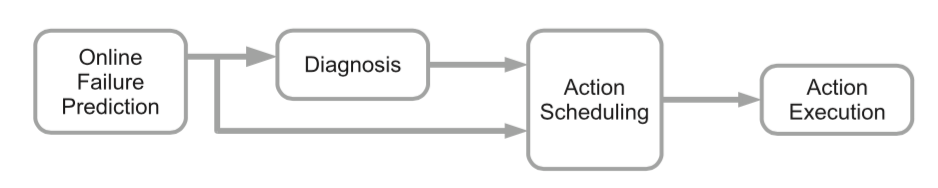
\includegraphics[width=#1]{proactiveFaultManagement}
     \caption[Proactive Fault Management~\cite{salfnerSurvey}]{The stages of
     proactive fault management~\cite{salfnerSurvey}.}
     \label{fig:proactiveFaultManagement}
 \end{center}
\end{figure}
}

\newcommand{\figonlinePrediction}[1]{\begin{figure}
 \begin{center}
    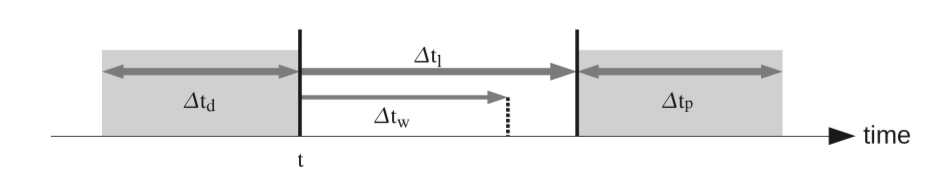
\includegraphics[width=#1]{onlinePrediction}
     \caption[\ac{OFP}~\cite{salfnerSurvey}]{The timeline for
     \ac{OFP}~\cite{salfnerSurvey}.}
     \label{fig:onlinePrediction}
 \end{center}
\end{figure}
}

\newcommand{\figfailureFlowDiagram}[1]{\begin{figure}
 \begin{center}
    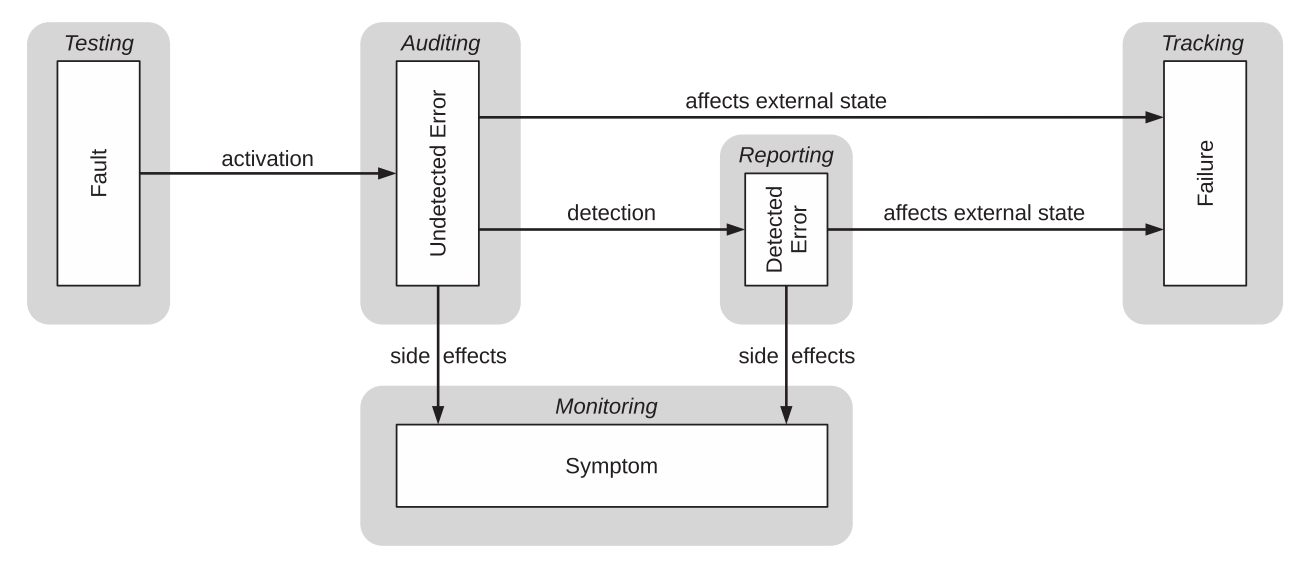
\includegraphics[width=#1]{failureFlowDiagram}
     \caption[Failure Flow Diagram~\cite{salfnerSurvey}]{How faults and errors
     evolve into failure with the associated methods for detection represented
     by enclosing gray boxes~\cite{salfnerSurvey}.}
     \label{fig:failureFlowDiagram}
 \end{center}
 %\vspace{-0.2 in}
\end{figure}
}

\newcommand{\figROC}[1]{\begin{figure}
 \begin{center}
    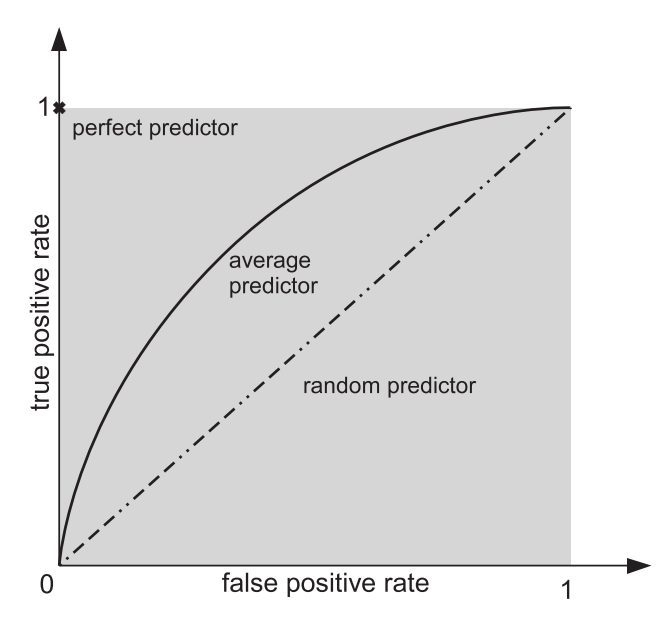
\includegraphics[width=#1]{ROC}
     \caption[Sample \ac{ROC} Plots~\cite{salfnerSurvey}]{\ac{ROC} plots of
     perfect, average, and random predictors~\cite{salfnerSurvey}.}
     \label{fig:ROC}
 \end{center}
\end{figure}
}

\newcommand{\figprecisionRecallCurve}[1]{\begin{figure}
 \begin{center}
    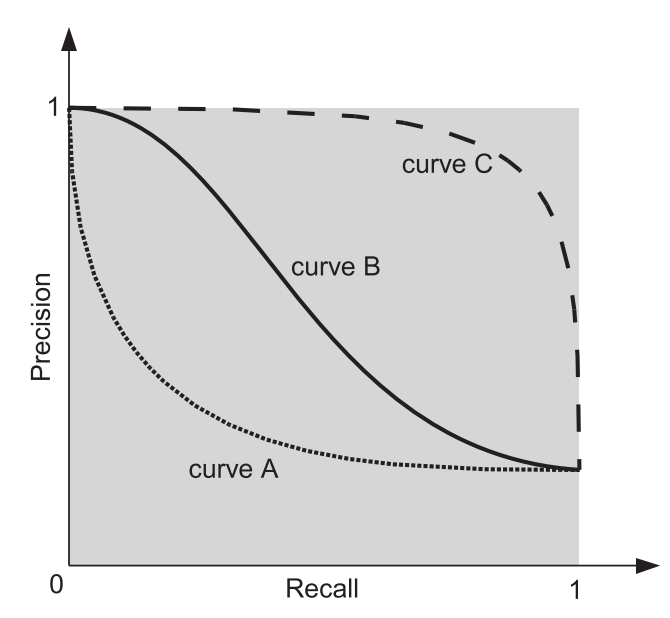
\includegraphics[width=#1]{precisionRecallCurve}
     \caption[Sample Precision/Recall Curves~\cite{salfnerSurvey}]{Sample
     precision/recall curves~\cite{salfnerSurvey}.  Curve $A$ represents a
     poorly performing predictor, curve $B$ an average predictor, and curve $C$
     an exceptional predictor.}
     \label{fig:precisionRecallCurve}
 \end{center}
\end{figure}
}

\newcommand{\figpatternRecognition}[1]{\begin{figure}
 \begin{center}
    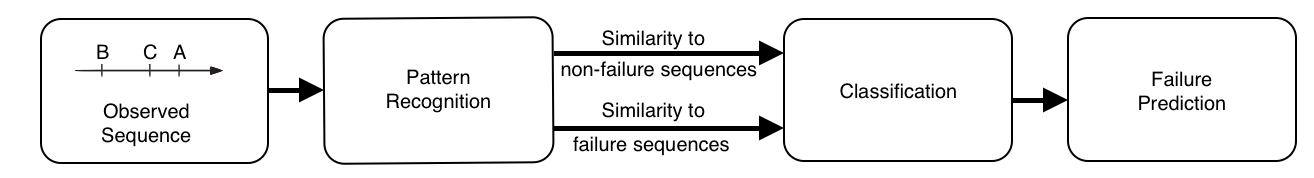
\includegraphics[width=#1]{patternRecognition}
     \caption[Pattern recognition in reported errors~\cite{salfnerSurvey}]{How
     pattern recognition is accomplished in reported
     errors~\cite{salfnerSurvey}.}
     \label{fig:patternRecognition}
 \end{center}
\end{figure}
}

\newcommand{\figAFP}[1]{\begin{figure}[t!h]
 \begin{center}
    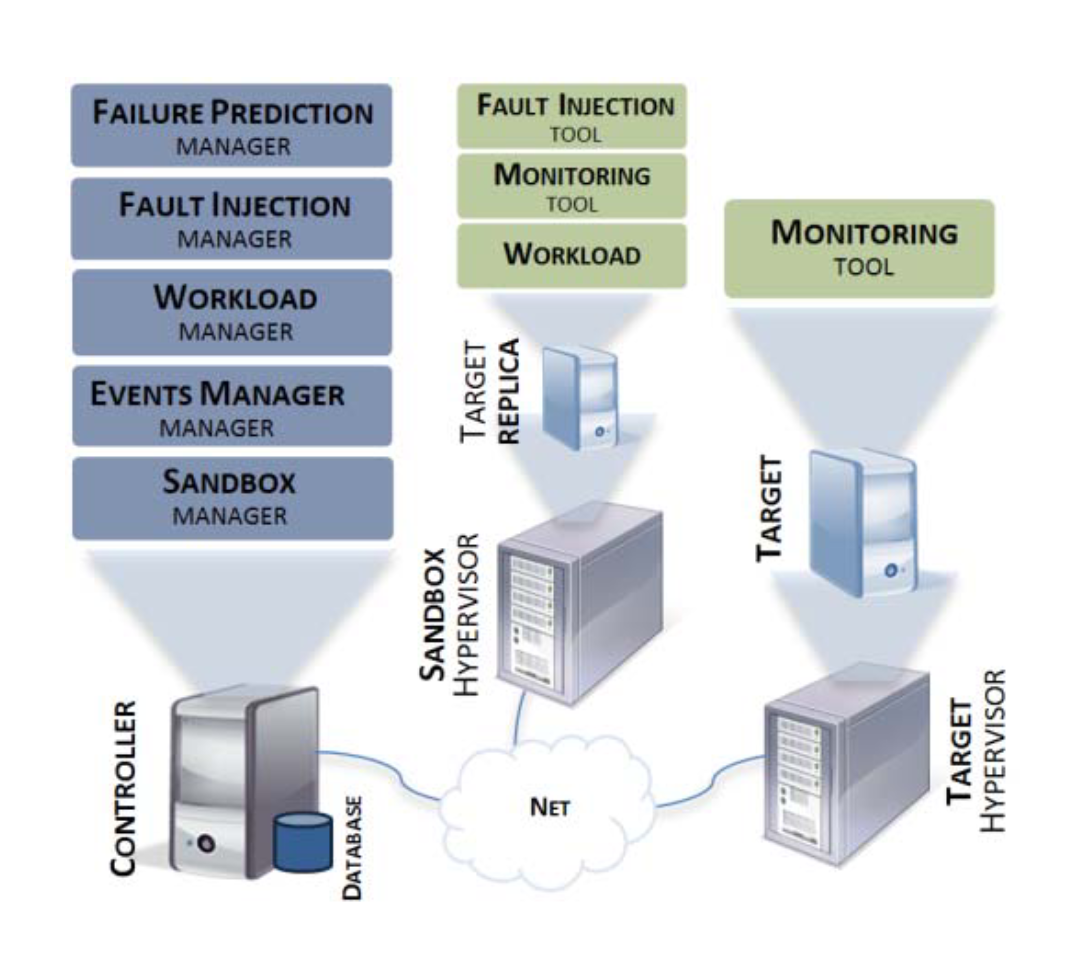
\includegraphics[width=#1]{AFP}
     \caption{The \ac{AFP} framework~\cite{irrera2015}.}
     \label{fig:AFP}
 \end{center}
\end{figure}
}

\definecolor{airforceblue}{rgb}{0.36, 0.54, 0.66}
\definecolor{armygreen}{rgb}{0.29, 0.33, 0.13}

\newcommand{\figannotatedAFPcolor}{\begin{figure}
 \begin{center}
     \begin{overpic}[width=5in,scale=.25]{annotatedAFPcolor}
       \put(8,0){
         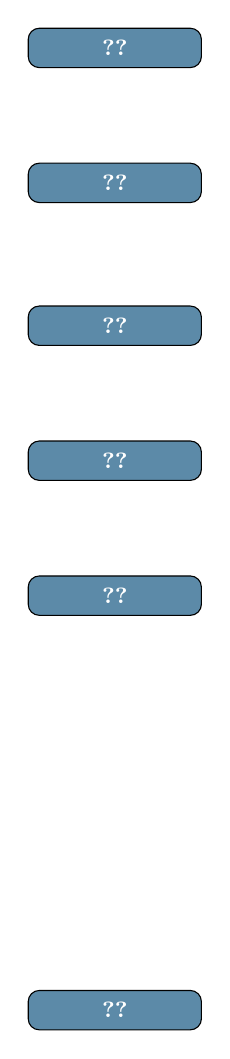
\begin{tikzpicture}
           [node font=\footnotesize, label/.style={rectangle, draw,
           fill=airforceblue, text width=2cm, text badly centered, minimum
           height=0.5cm, rounded corners}]

           \node[label] (FPMgr)
             {\textcolor{white}{\ref{sec:failurePrediction}}};
           \node[label, below=1.2cm of FPMgr] (FIMgr) 
             {\textcolor{white}{\ref{sec:faultInjectionMgr}}};
           \node[label, below=1.3cm of FIMgr] (WMgr) 
             {\textcolor{white}{\ref{sec:workloadMgr}}};
           \node[label, below=1.2cm of WMgr] (EMMgr) 
             {\textcolor{white}{\ref{sec:eventsManagerMgr}}};
           \node[label, below=1.2cm of EMMgr] (SMgr) 
             {\textcolor{white}{\ref{sec:sandboxMgr}}};
           \node[label, below=4.75cm of SMgr] (Controller) 
             {\textcolor{white}{\ref{sec:controller}}};
         \end{tikzpicture}
       }

       \put(40,60.5){
         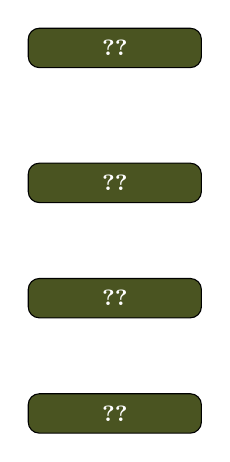
\begin{tikzpicture}
           [node font=\footnotesize, label/.style={rectangle, draw,
           fill=armygreen, text width=2cm, text badly centered, minimum
           height=0.5cm, rounded corners}]

           \node[label] (Sandbox)
             {\textcolor{white}{\ref{sec:sandbox}}};
           \node[label, below=1.2cm of Sandbox] (SBFITool)
             {\textcolor{white}{\ref{sec:faultInjectionTool}}};
           \node[label, below=0.95cm of SBFITool] (SBMTool) 
             {\textcolor{white}{\ref{sec:sandboxMonitoringTool}}};
           \node[label, below=0.95cm of SBMTool] (SBWorkload) 
             {\textcolor{white}{\ref{sec:sandboxWorkload}}};
         \end{tikzpicture}
       }

       \put(66,0){
         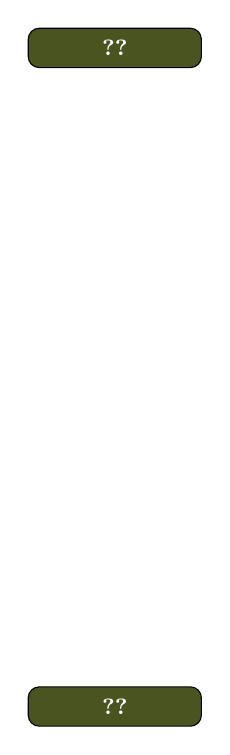
\begin{tikzpicture}
           [node font=\footnotesize, label/.style={rectangle, draw,
           fill=armygreen, text width=2cm, text badly centered, minimum
           height=0.5cm, rounded corners}]

           \node[label] (MonTool)
             {\textcolor{white}{\ref{sec:targetMonitoringTool}}};
           \node[label, below=7.85cm of MonTool] (Target)
             {\textcolor{white}{\ref{sec:target}}};
         \end{tikzpicture}
       }
     \end{overpic}
     \caption[Annotated \ac{AFP} Framework~\cite{irrera2015}]{The \ac{AFP}
     framework implementation~\cite{irrera2015} with modified components
     highlighted.}
     \label{fig:annotatedAFP}
 \end{center}
\end{figure}
}

\newcommand{\figannotatedAFP}{\begin{figure}
 \begin{center}
     \begin{overpic}[width=5in,scale=.25]{annotatedAFP}
       \put(8,0){
         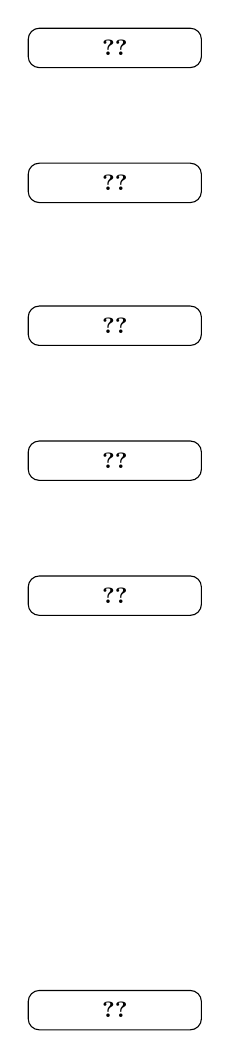
\begin{tikzpicture}
           [node font=\footnotesize, label/.style={rectangle, draw,
           fill=white, text width=2cm, text badly centered, minimum
           height=0.5cm, rounded corners}]

           \node[label] (FPMgr)
             {\textcolor{black}{\ref{sec:failurePrediction}}};
           \node[label, below=1.2cm of FPMgr] (FIMgr) 
             {\textcolor{black}{\ref{sec:faultInjectionMgr}}};
           \node[label, below=1.3cm of FIMgr] (WMgr) 
             {\textcolor{black}{\ref{sec:workloadMgr}}};
           \node[label, below=1.2cm of WMgr] (EMMgr) 
             {\textcolor{black}{\ref{sec:eventsManagerMgr}}};
           \node[label, below=1.2cm of EMMgr] (SMgr) 
             {\textcolor{black}{\ref{sec:sandboxMgr}}};
           \node[label, below=4.75cm of SMgr] (Controller) 
             {\textcolor{black}{\ref{sec:controller}}};
         \end{tikzpicture}
       }

       \put(40,60.5){
         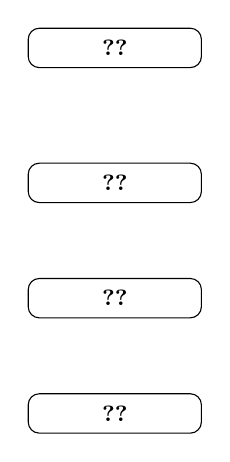
\begin{tikzpicture}
           [node font=\footnotesize, label/.style={rectangle, draw,
           fill=white, text width=2cm, text badly centered, minimum
           height=0.5cm, rounded corners}]

           \node[label] (Sandbox)
             {\textcolor{black}{\ref{sec:sandbox}}};
           \node[label, below=1.2cm of Sandbox] (SBFITool)
             {\textcolor{black}{\ref{sec:faultInjectionTool}}};
           \node[label, below=0.95cm of SBFITool] (SBMTool) 
             {\textcolor{black}{\ref{sec:sandboxMonitoringTool}}};
           \node[label, below=0.95cm of SBMTool] (SBWorkload) 
             {\textcolor{black}{\ref{sec:sandboxWorkload}}};
         \end{tikzpicture}
       }

       \put(66,0){
         \begin{tikzpicture}
           [node font=\footnotesize, label/.style={rectangle, draw,
           fill=white, text width=2cm, text badly centered, minimum
           height=0.5cm, rounded corners}]

           \node[label] (MonTool)
             {\textcolor{black}{\ref{sec:targetMonitoringTool}}};
           \node[label, below=7.85cm of MonTool] (Target)
             {\textcolor{black}{\ref{sec:target}}};
         \end{tikzpicture}
       }
     \end{overpic}
     \caption[Annotated \ac{AFP} Framework~\cite{irrera2015}]{The \ac{AFP}
     framework implementation~\cite{irrera2015} with modified components
     highlighted.}
     \label{fig:annotatedAFP}
 \end{center}
\end{figure}
}

\newcommand{\figTrainingPhase}[1]{\begin{figure}[h!t]
 \begin{center}
  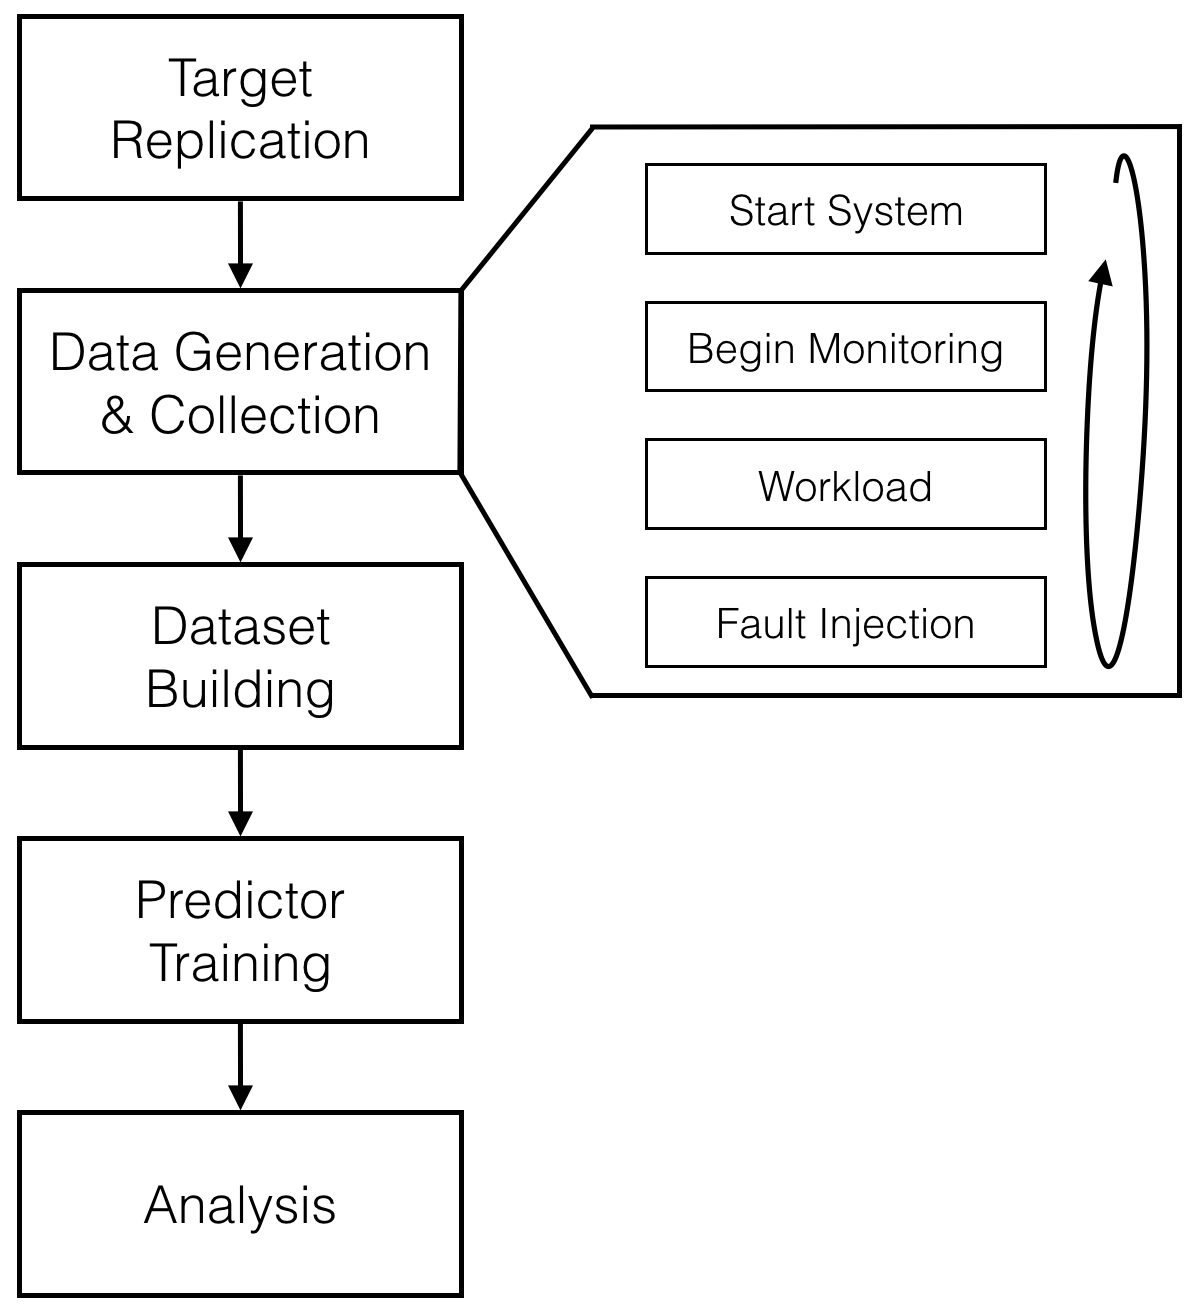
\includegraphics[width=#1]{TrainingPhase}
  \caption[\ac{AFP} Training Phase~\cite{irrera2015}]{The flow of the major
  steps involved in the \ac{AFP} framework training phase~\cite{irrera2015}.}
  \label{fig:TrainingPhase}
 \end{center}
\end{figure}
}

\newcommand{\figExecutionPhase}[1]{\begin{figure}[h!t]
  \begin{center}
    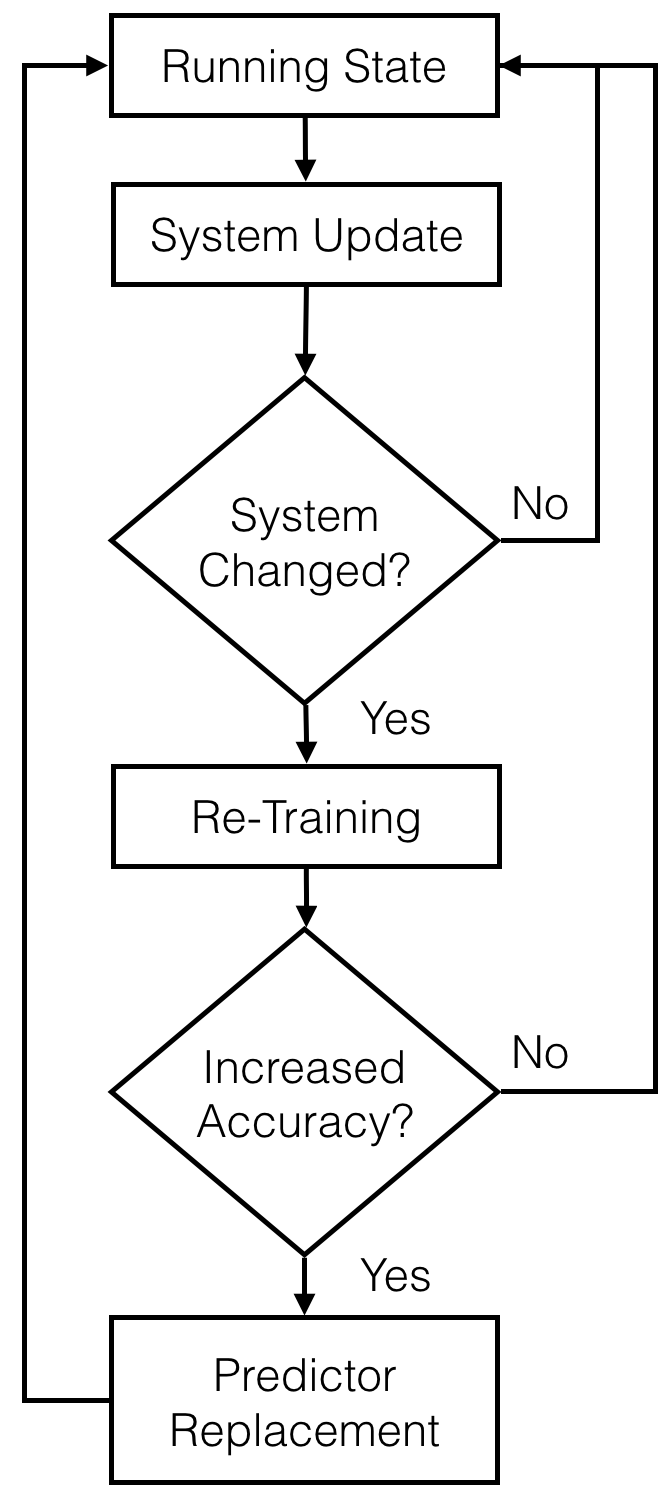
\includegraphics[width=#1]{ExecutionPhase}
    \caption[\ac{AFP} Execution Phase~\cite{irrera2015}]{The flow of the major
    steps involved in the \ac{AFP} framework execution
    phase~\cite{irrera2015}.}
    \label{fig:ExecutionPhase}
  \end{center}
\end{figure}
}


\newcommand{\figExecutionPhaseHoriz}[1]{\begin{figure}
  \begin{center}
    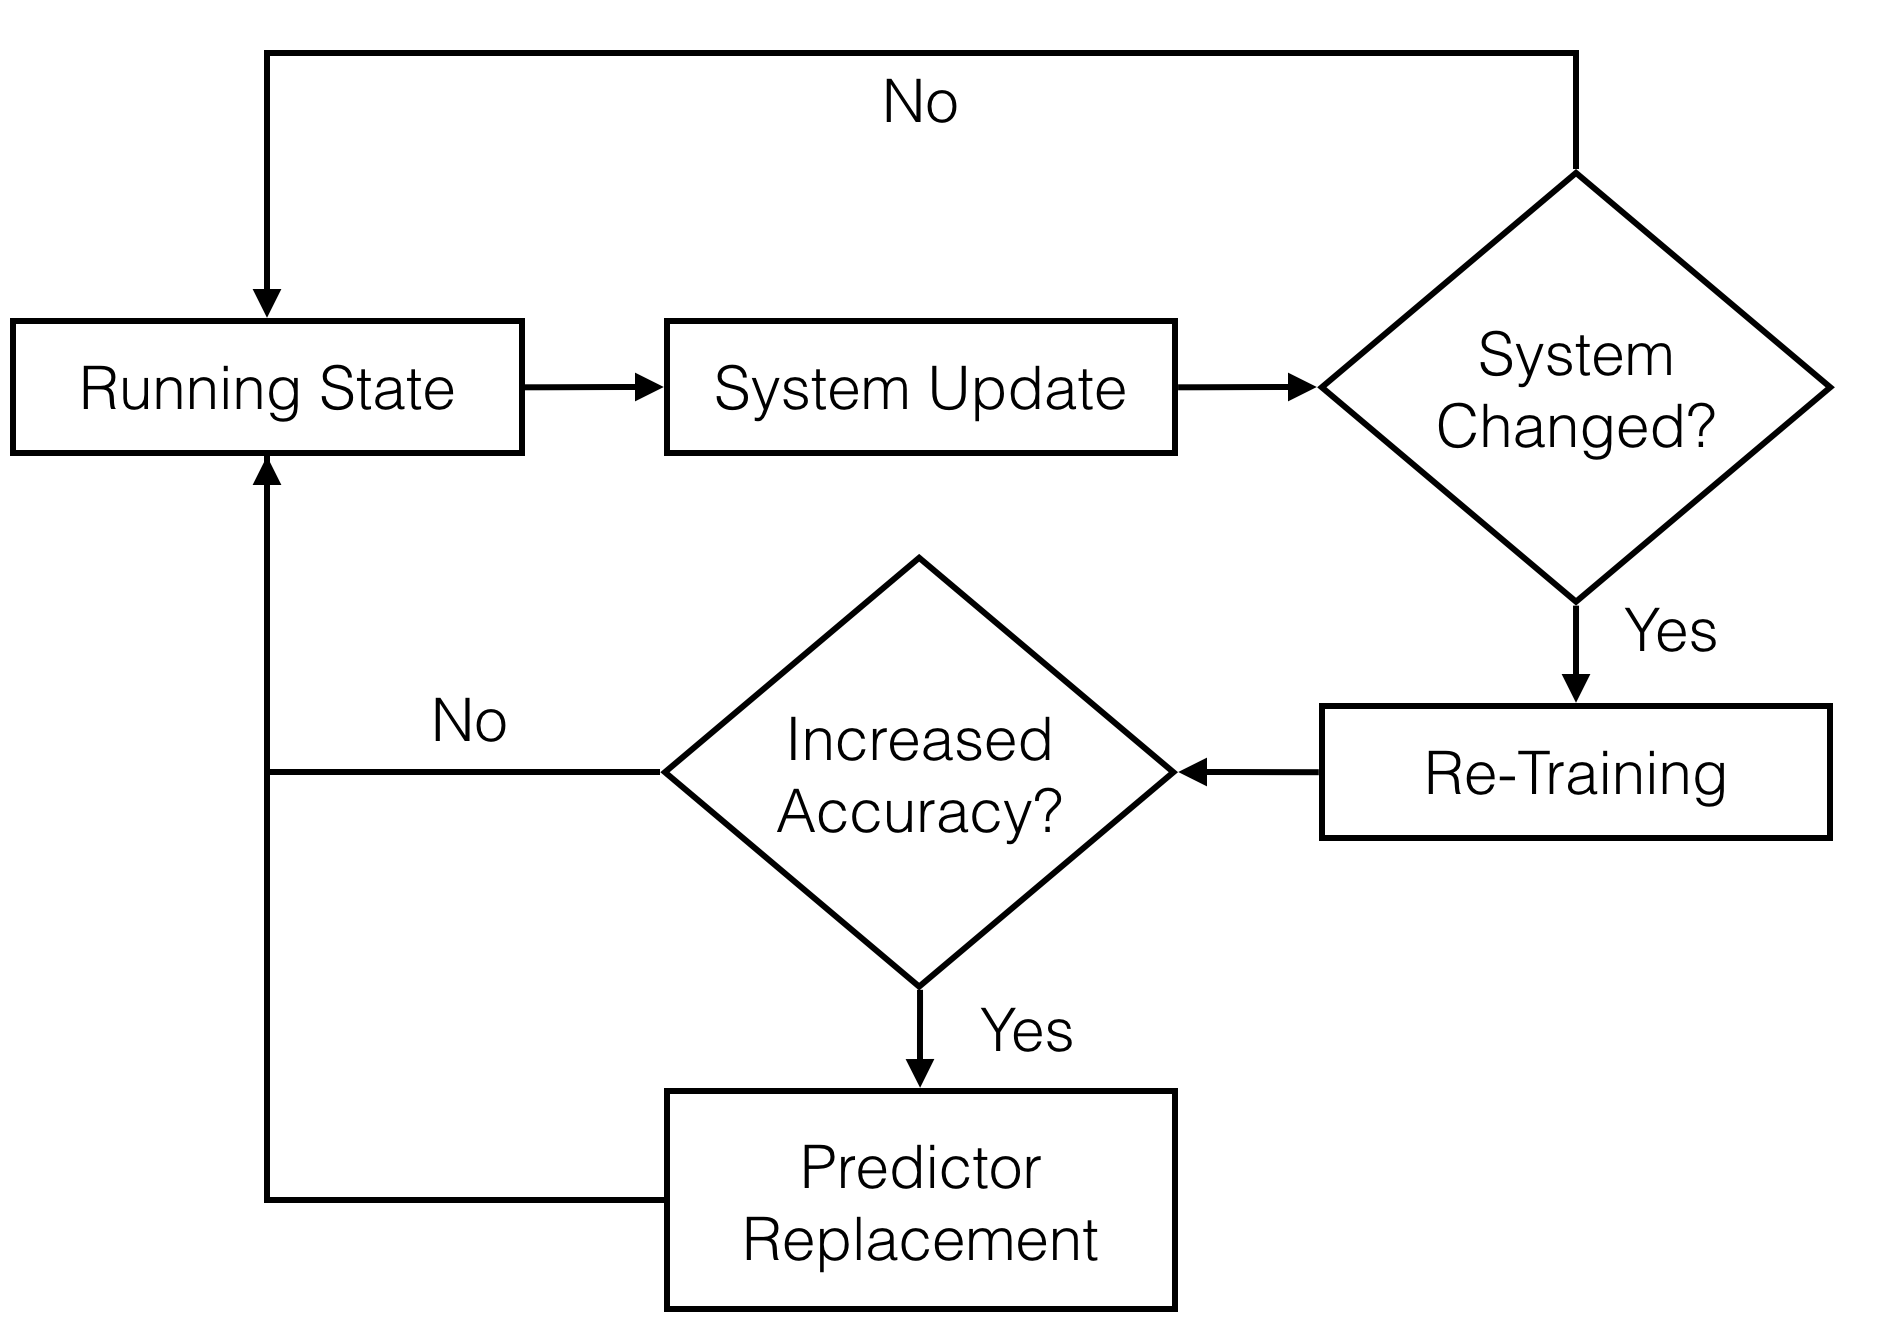
\includegraphics[width=#1]{ExecutionPhaseHoriz}
    \caption[\ac{AFP} Execution Phase~\cite{irrera2015}]{The flow of the major
    steps involved in the \ac{AFP} framework execution
    phase~\cite{irrera2015}.}
    \label{fig:ExecutionPhaseHoriz}
  \end{center}
\end{figure}
}

\newcommand{\figAuthDCPPS}[1]{\begin{figure}
 \begin{center}
  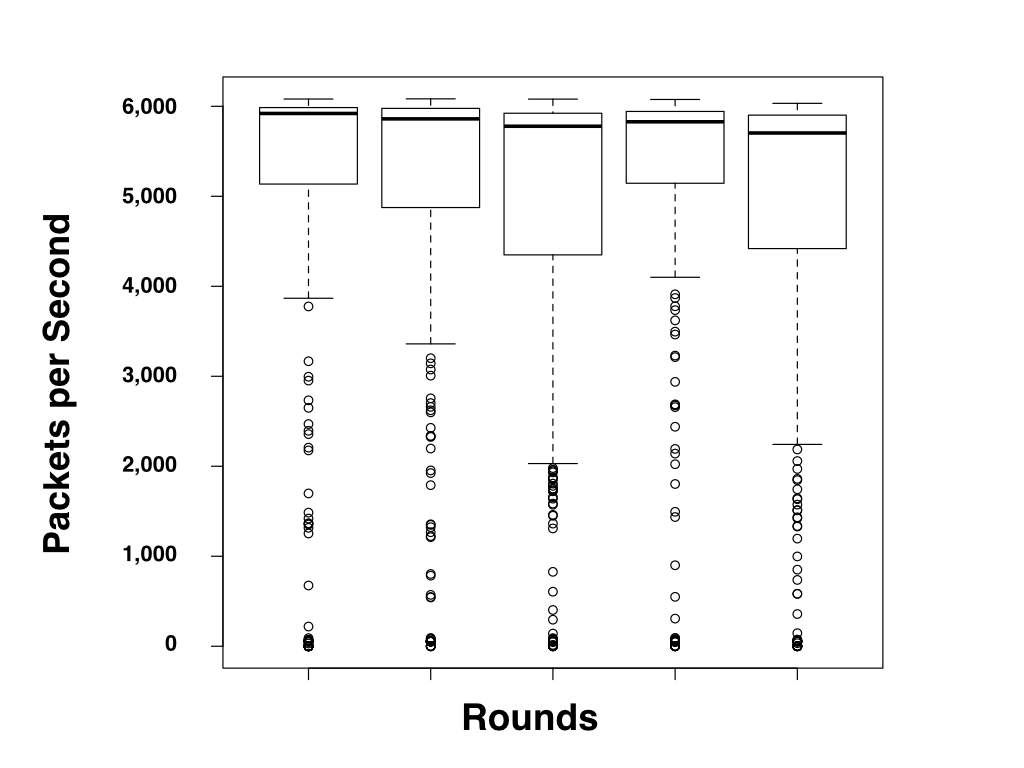
\includegraphics[width=#1]{DPLG/authDCPPS}
  \caption[Domain Controller Packets per Second]{How many packets per second
  were sent or received by the domain controller across all five rounds of the
  first test.  In each test, we captured approximately 1.8 million packets.}
  \label{fig:authDCPPS}
 \end{center}
\end{figure}
}

\newcommand{\figAuthClientPPS}[1]{\begin{figure}
 \begin{center}
  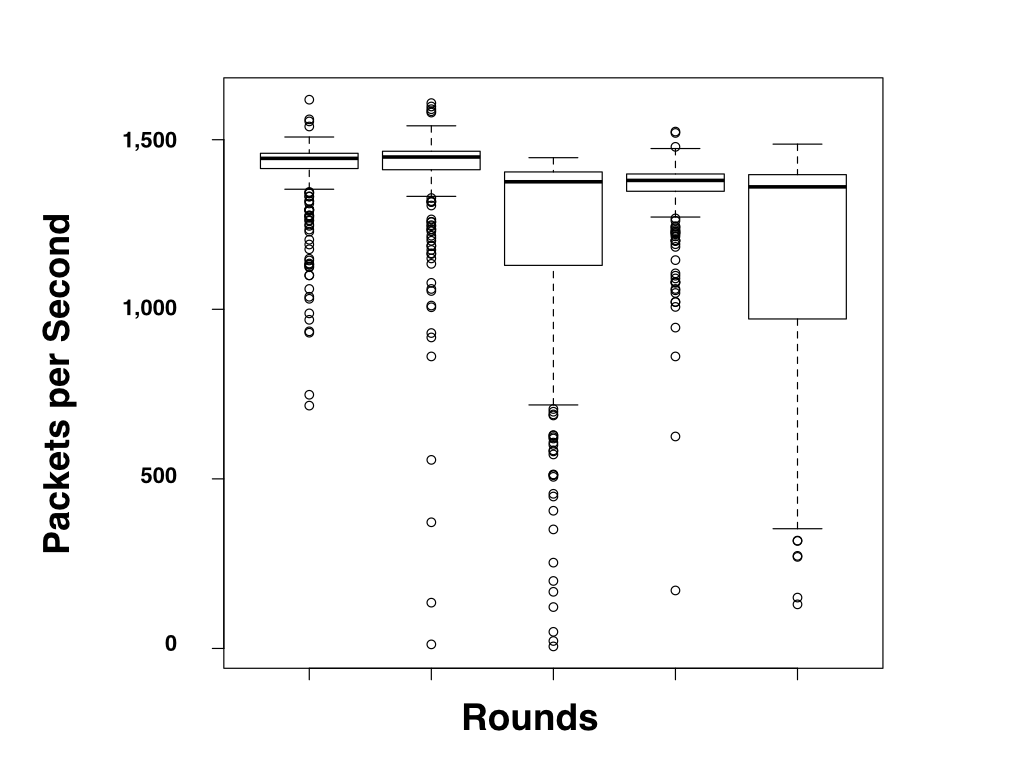
\includegraphics[width=#1]{DPLG/authClientPPS}
  \caption[Client Packets per Second]{How many packets per second were sent or
  received by one of the clients across all five rounds of the first test.}
  \label{fig:authClientPPS}
 \end{center}
\end{figure}
}

\newcommand{\figAuthDCMetrics}[1]{\begin{figure}
 \begin{center}
  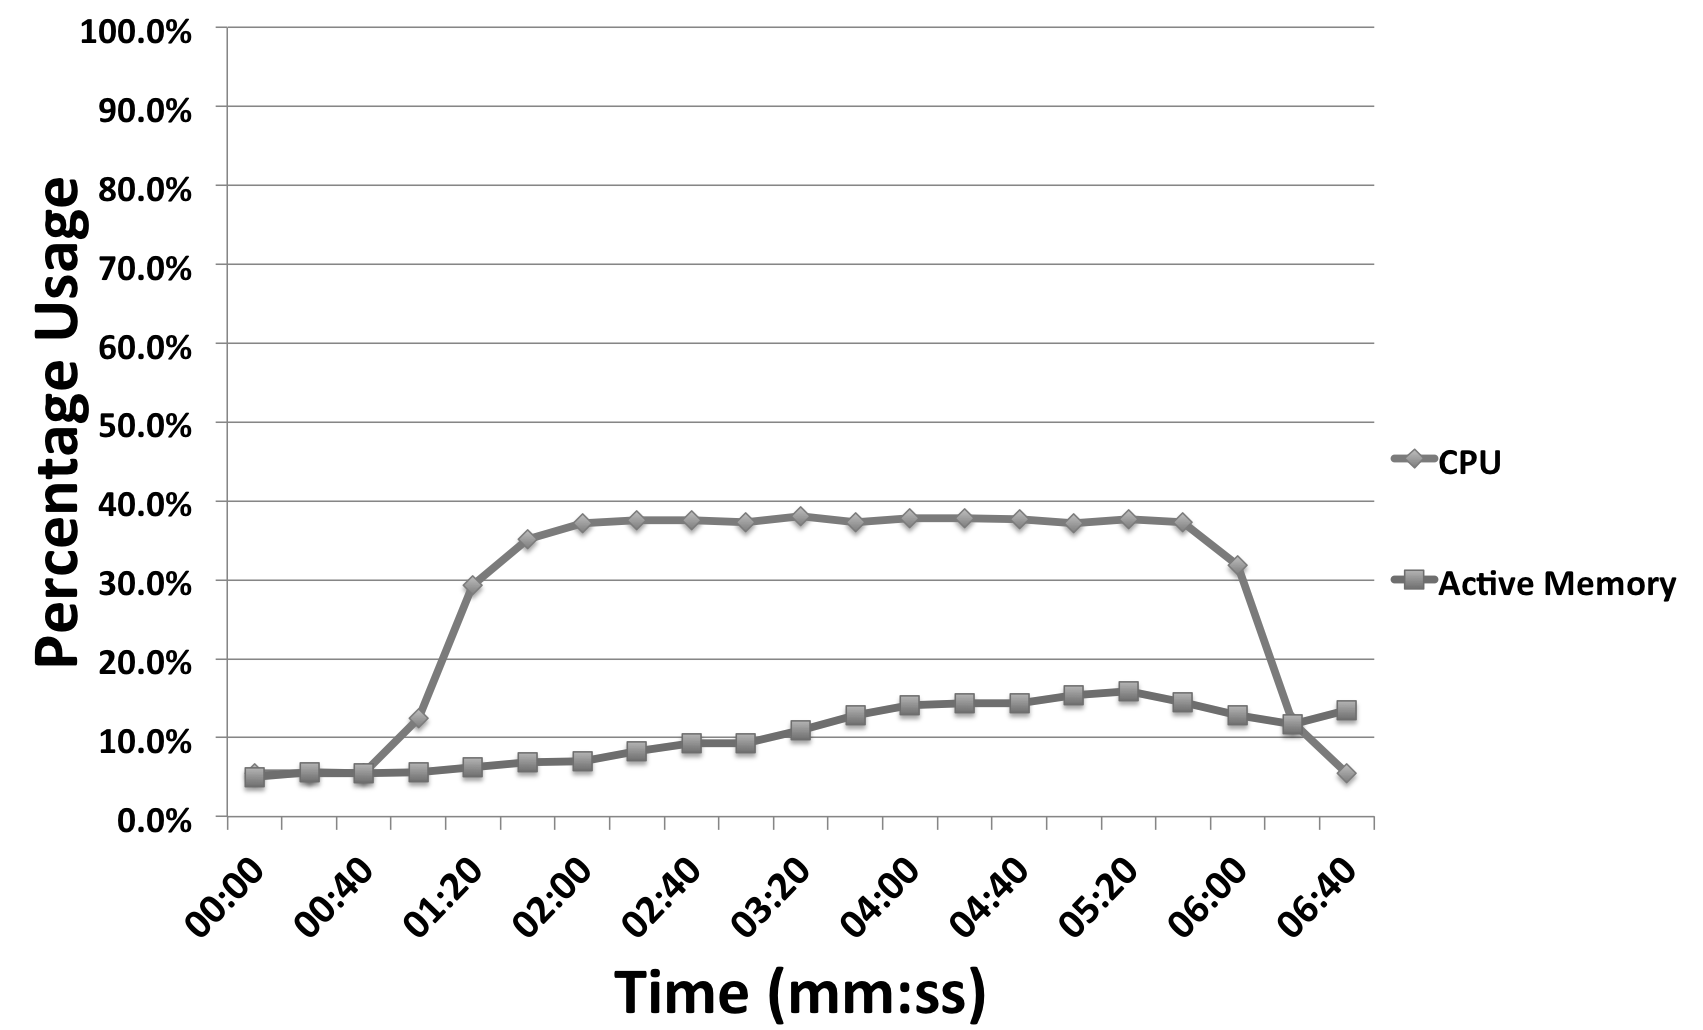
\includegraphics[width=#1]{DPLG/authDCMetrics}
  \caption[Test 1:  Domain Controller Performance]{Domain controller CPU and
  memory utilization during the first test.}
  \label{fig:authDCMetrics}
 \end{center}
\end{figure}
}

\newcommand{\figOFPTaxonomy}[1]{\begin{figure}
 \begin{center}
  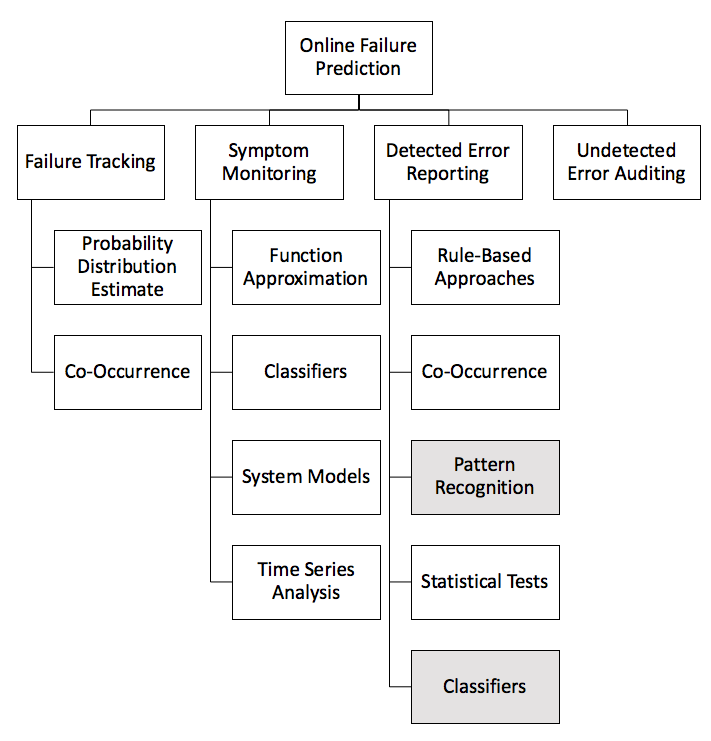
\includegraphics[width=#1]{OFPTaxonomy}
  \caption[Taxonomy of \ac{OFP} Approaches]{Taxonomy of approaches to online
  failure prediction~\cite{salfnerSurvey}.  The two categories into which this
  research falls are highlighted.}
  \label{fig:OFPTaxonomy}
 \end{center}
\end{figure}
}

\newcommand{\figMemLeakROC}[1]{\begin{figure}
 \begin{center}
  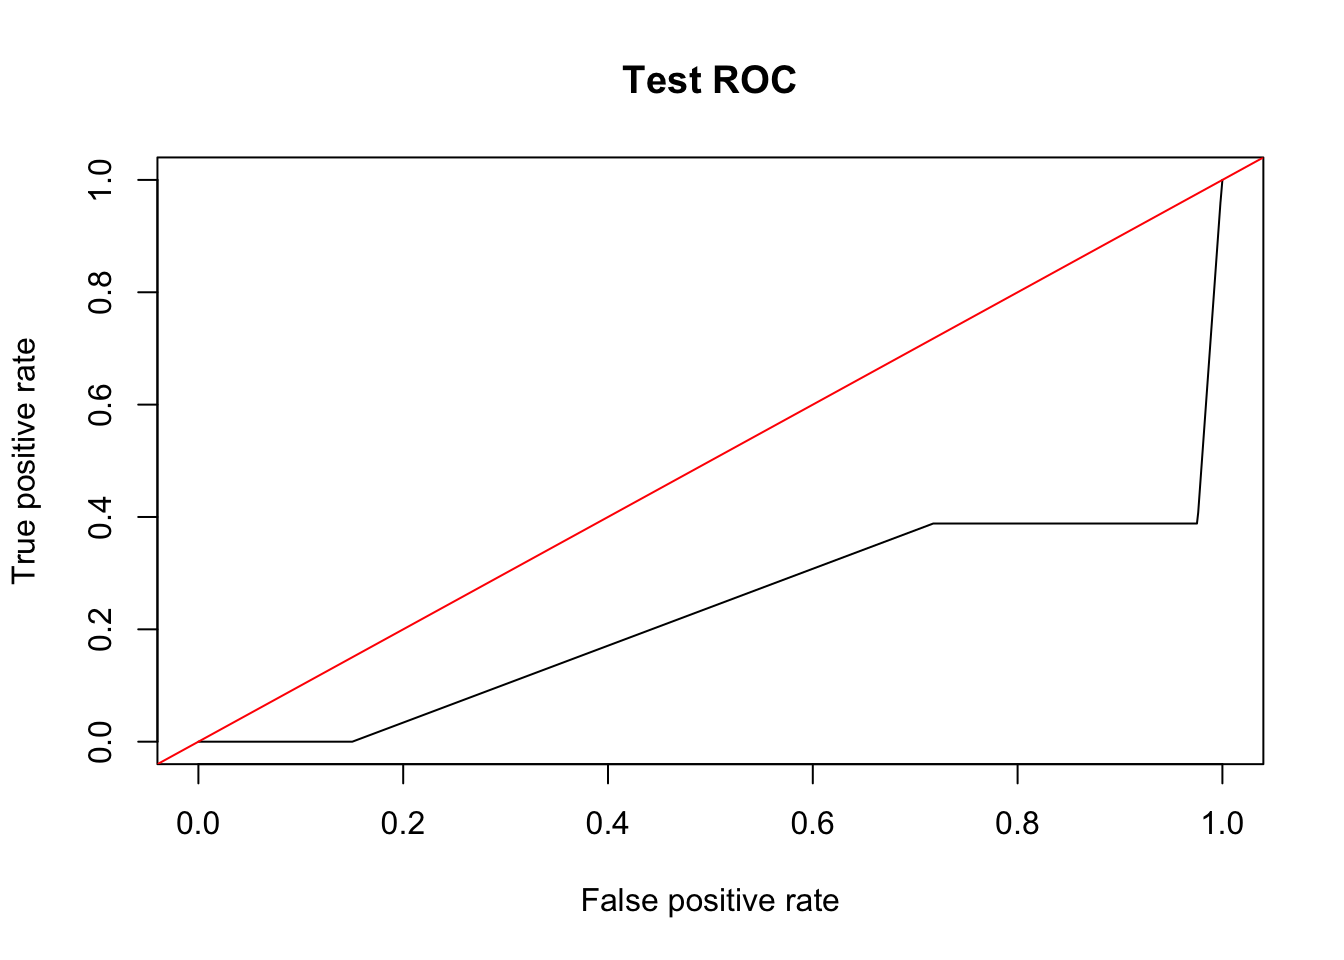
\includegraphics[width=#1]{MemLeakROC}
  \caption[\ac{SVM} Memory Leak \ac{ROC} Curve]{\ac{SVM} memory leak test data
  \ac{ROC} curve.}
  \label{fig:memLeakROC}
 \end{center}
\end{figure}
}

\newcommand{\figMemLeakCompare}[1]{\begin{figure}
 \begin{center}
  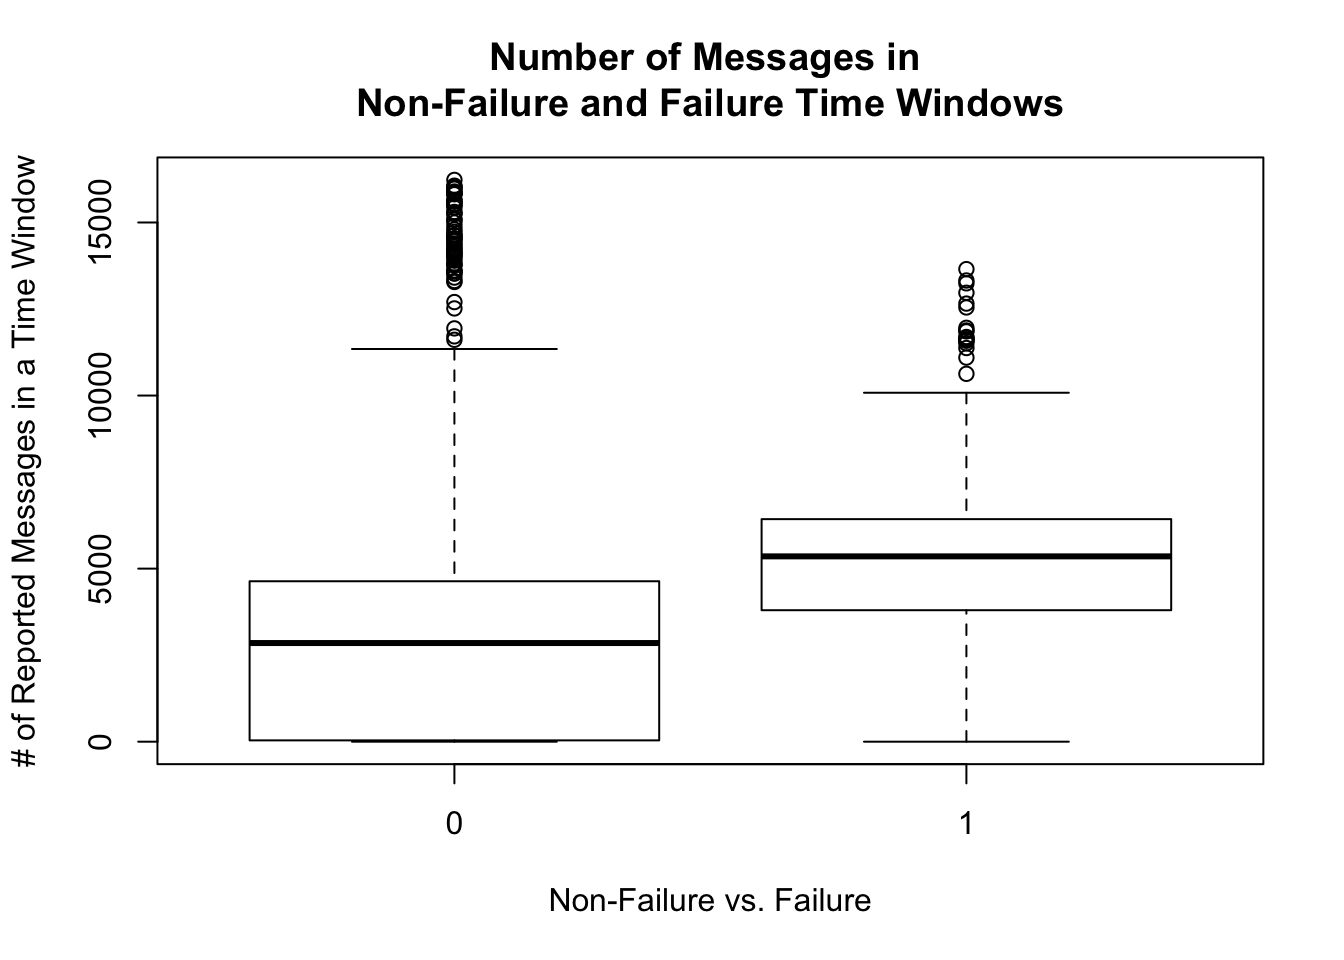
\includegraphics[width=#1]{MemLeakCompare}
  \caption[\ac{SVM} Memory Leak Performance Comparison]{Number of observations
  in a given thirty second time window where `1' represents a window during
  which failure occurred and `0' represents a window during which no failure
  occurred.}
  \label{fig:memLeakCompare}
 \end{center}
\end{figure}
}

%%%%   SMV   %%%%
% Pre-Update
\newcommand{\figMemLeakPreUpdateSVMPerf}{\begin{figure*}
  \centering
  \subfigure[Precision/Recall Curve.]{
    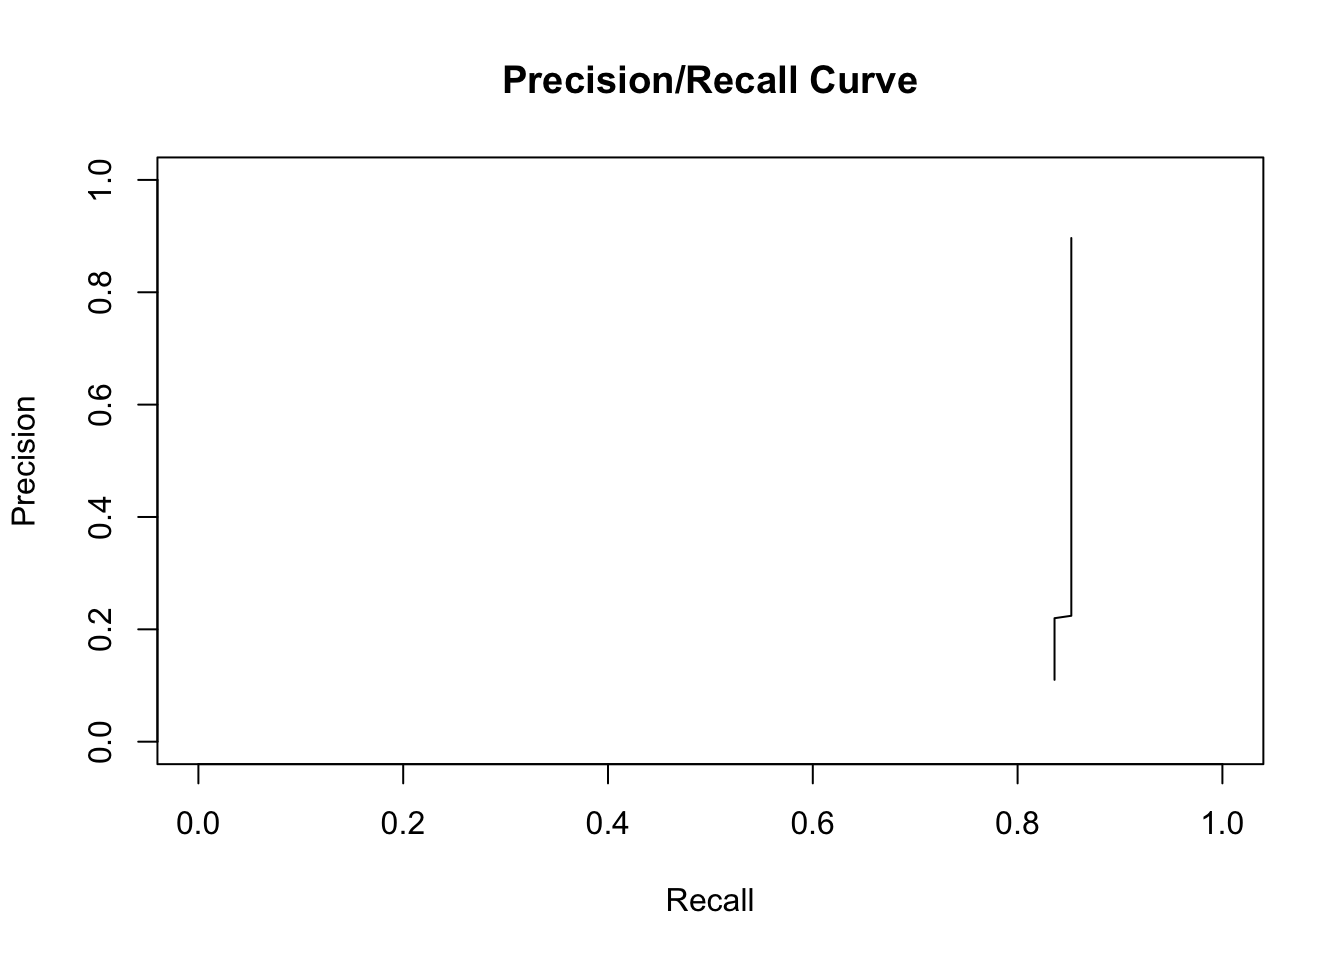
\includegraphics[width=0.45\textwidth]{results/pre-update/memleak/svm-prc}
  }
  \subfigure[\ac{ROC} Curve (\ac{AUC} = 0.8664).]{
    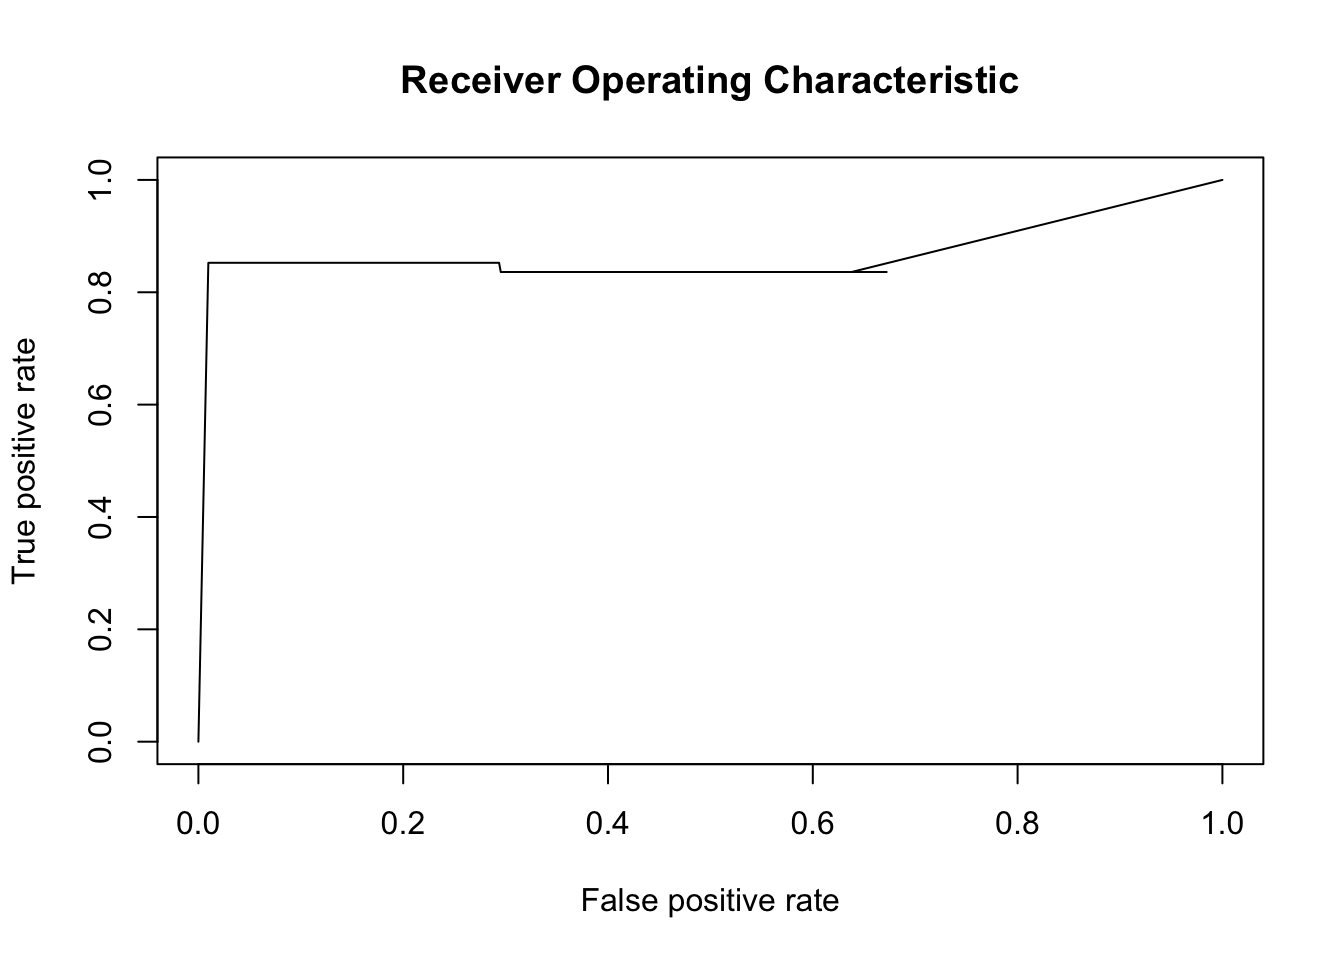
\includegraphics[width=0.45\textwidth]{results/pre-update/memleak/svm-roc}
  }
  \caption[Pre-Update, Memory Leak \ac{SVM} Performance]{Test data performance
  of the \ac{SVM} prediction method on failure data obtained by consuming all
  available memory until target application fails.}
  \label{fig:memLeakPreUpdateSVMPerf}
\end{figure*}
}

% Post-Update (old model)

% Post-Update New Model

%%%%   BOOSTING   %%%%
% Pre-Update
\newcommand{\figMemLeakPreUpdateBoostingPerf}{\begin{figure*}
  \centering
  \subfigure[Precision/Recall Curve.]{
    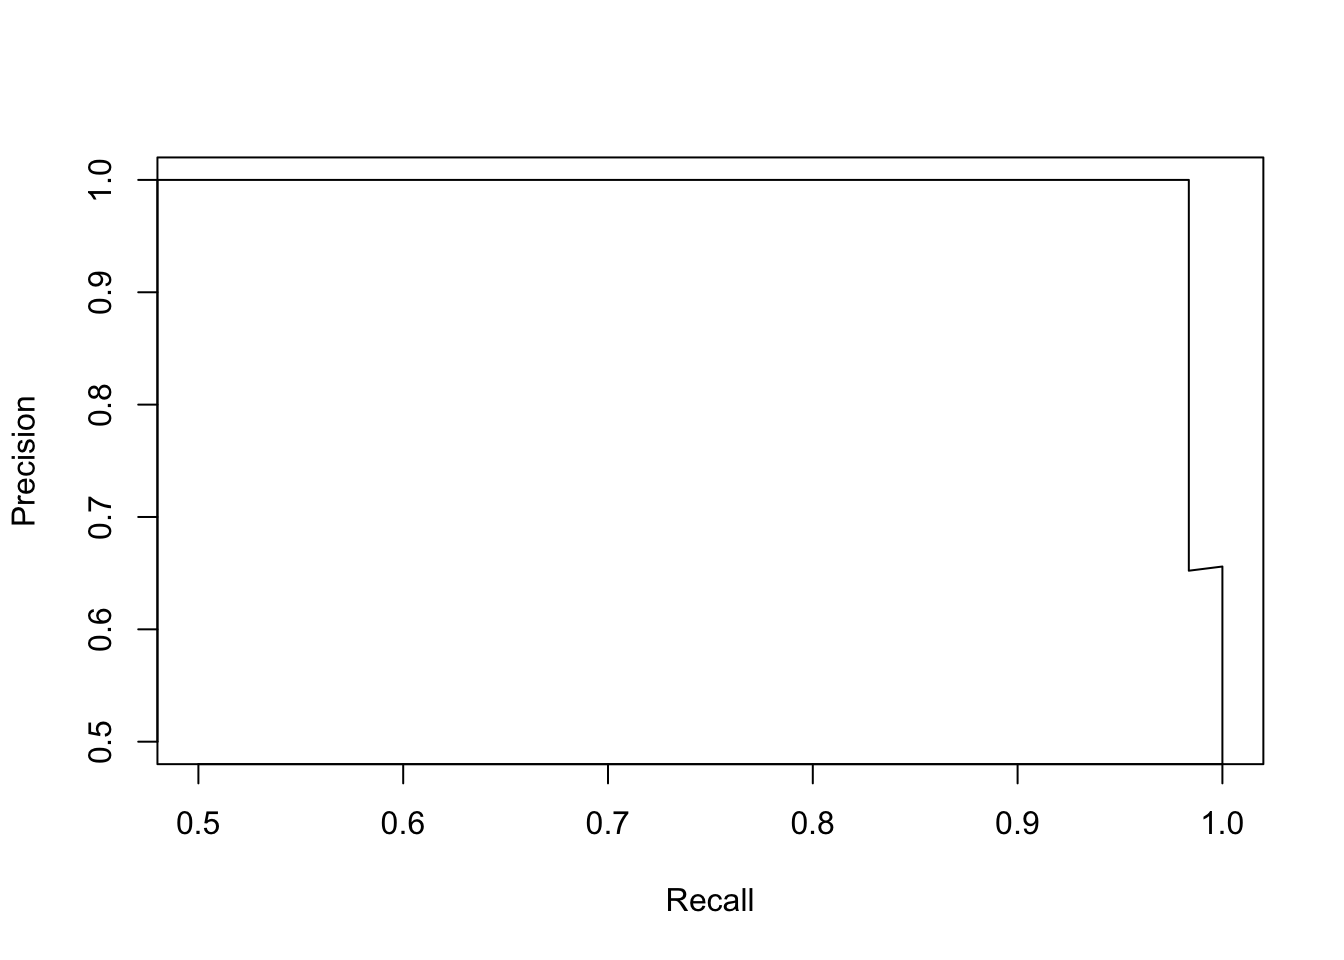
\includegraphics[width=0.45\textwidth]{results/pre-update/memleak/boosting-prc}
  }
  \subfigure[\ac{ROC} Curve (\ac{AUC} = 0.9984).]{
    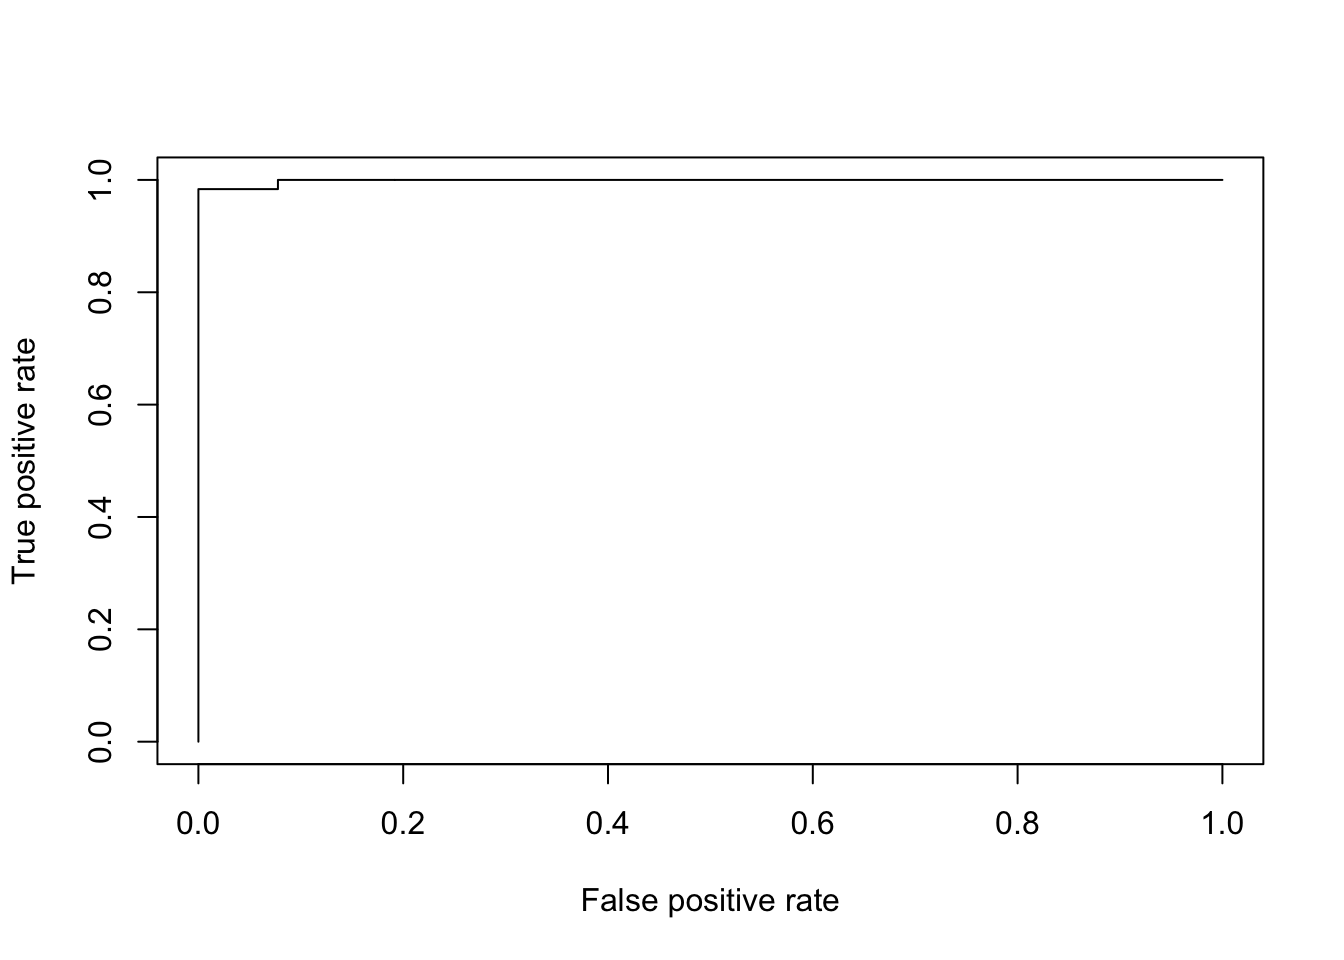
\includegraphics[width=0.45\textwidth]{results/pre-update/memleak/boosting-roc}
  }
  \caption[Pre-Update, Memory Leak Boosting Performance]{Test data performance
  of the boosting prediction method on failure data obtained by consuming all
  available memory until target application fails.}
  \label{fig:memLeakPreUpdateBoostingPerf}
\end{figure*}
}

% Post-Update (old model)
\newcommand{\figMemLeakPostUpdateSameBoostedModel}{\begin{figure*}
  \centering
  \subfigure[Precision/Recall Curve.]{
    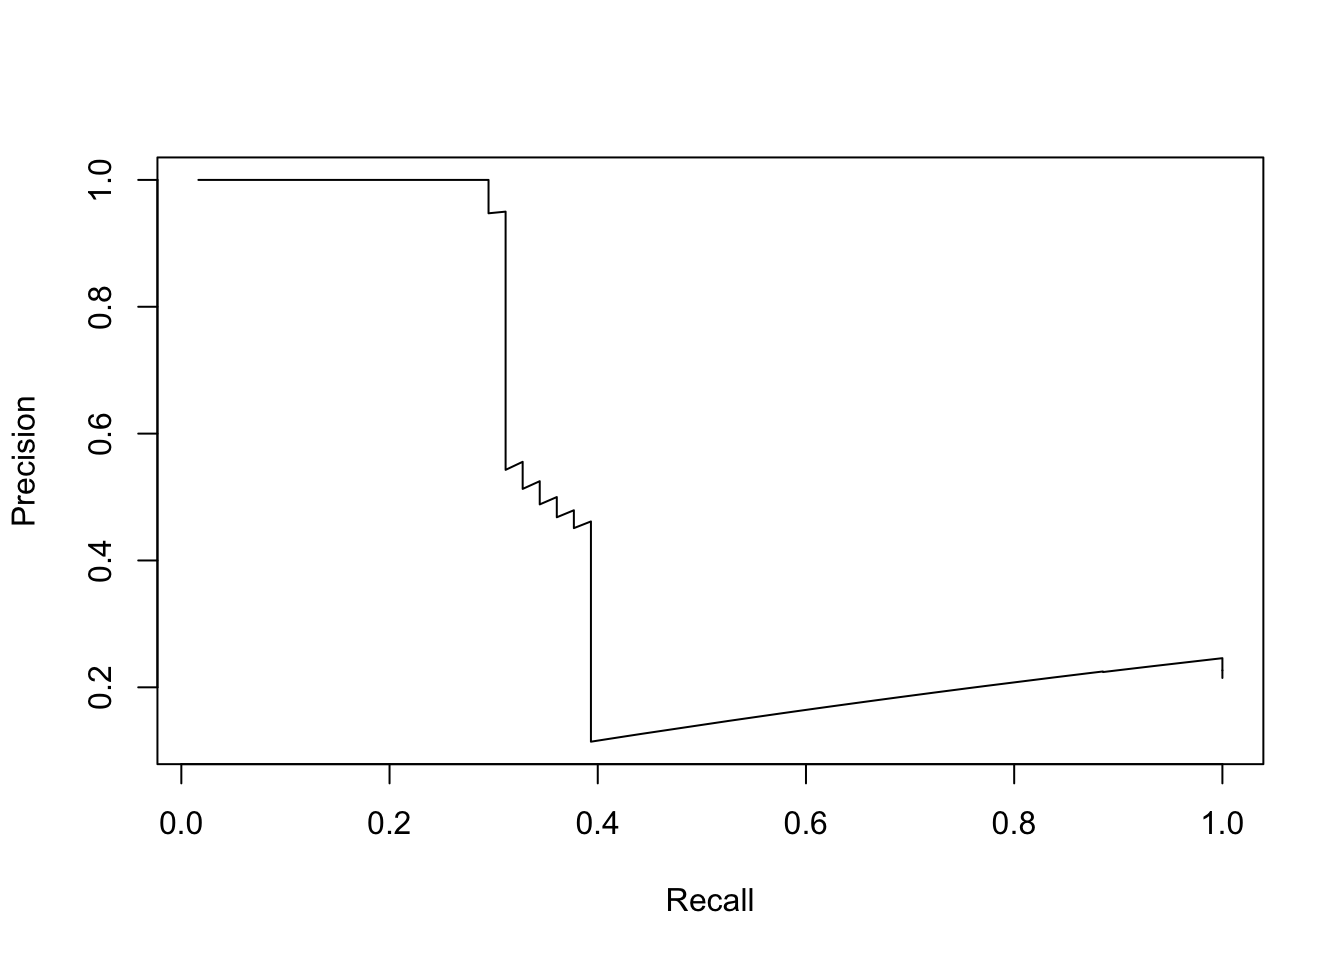
\includegraphics[width=0.45\textwidth]{results/post-update/memleak/boost-samemodel-prc}
  }
  \subfigure[\ac{ROC} Curve (\ac{AUC} = 0.4854).]{
    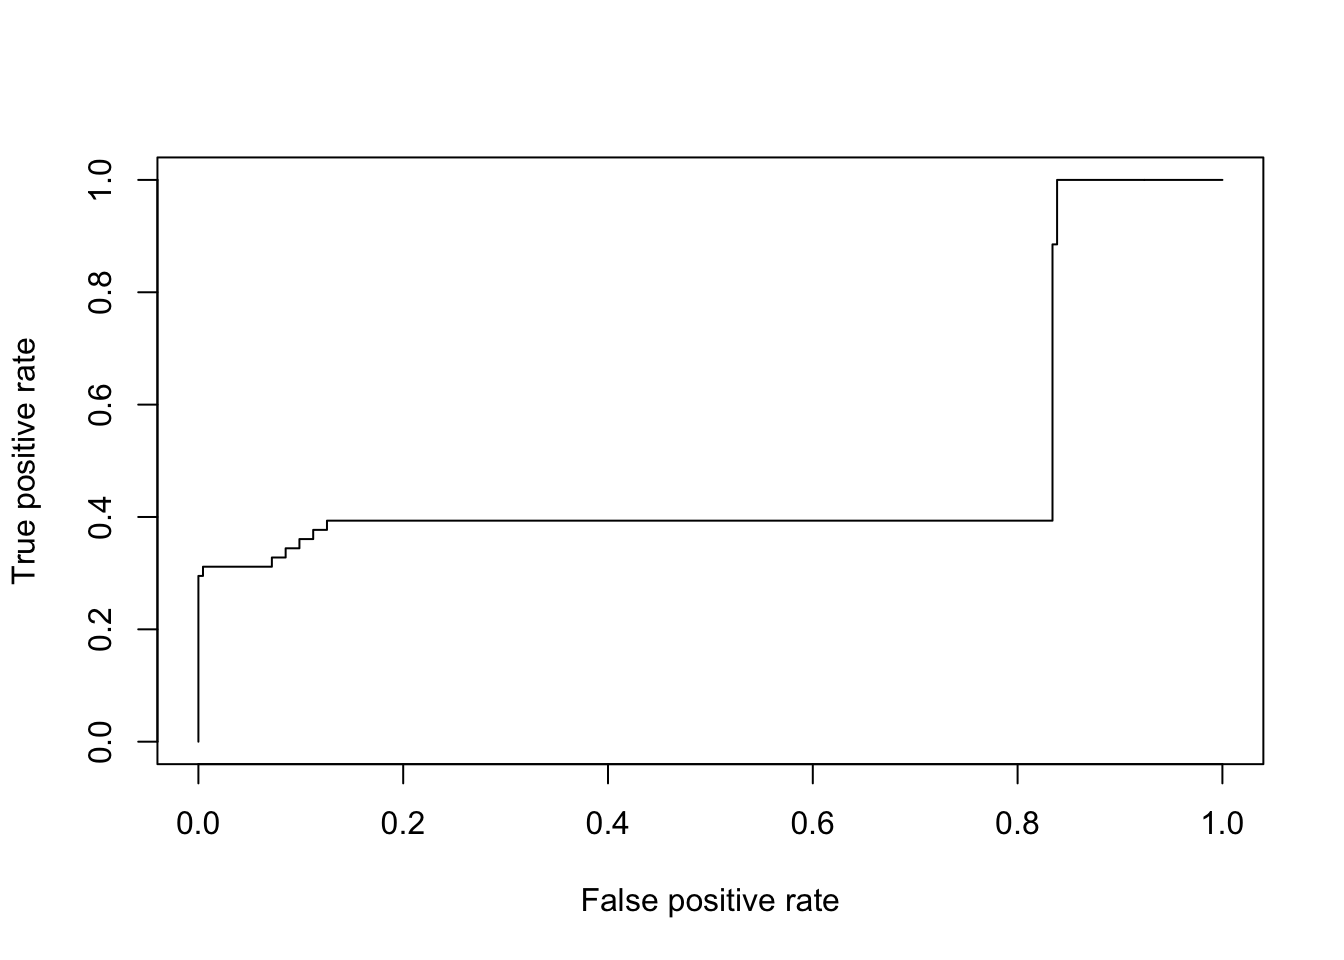
\includegraphics[width=0.45\textwidth]{results/post-update/memleak/boost-samemodel-roc}
  }
  \caption[Post-Update, Memory Leak Using Old Model Performance]{Performance of
  the boosting prediction method trained on failure data created before the
  software update obtained by consuming all available memory until target
  application fails.}
  \label{fig:memLeakPostUpdateSameBoostedModel}
\end{figure*}
}

% Post-Update New Model
\newcommand{\figMemLeakPostUpdateBoostingPerf}{\begin{figure*}
  \centering
  \subfigure[Precision/Recall Curve.]{
    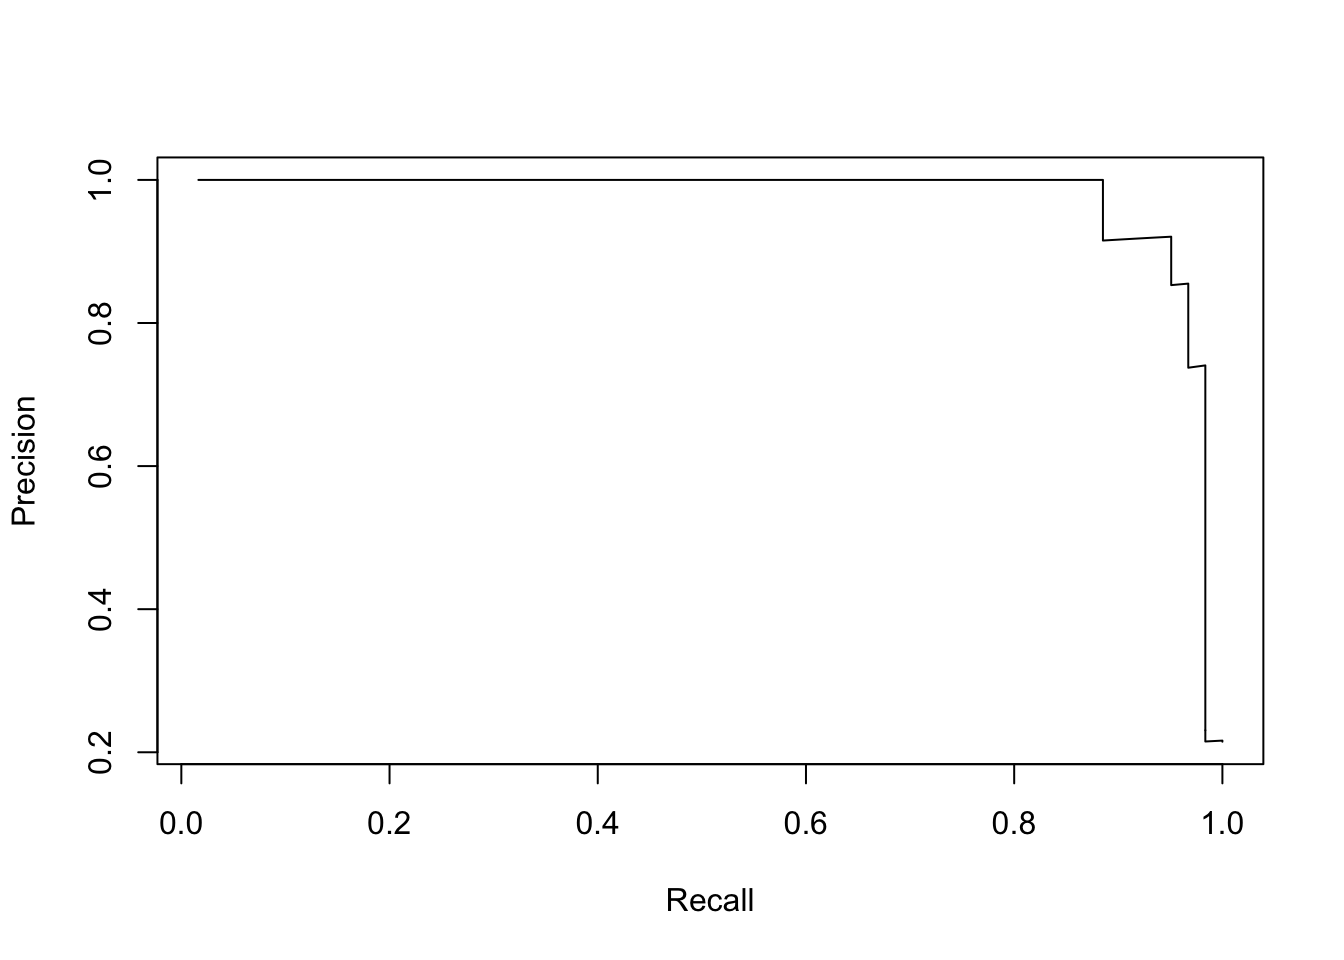
\includegraphics[width=0.45\textwidth]{results/post-update/memleak/boost-prc}
  }
  \subfigure[\ac{ROC} Curve (\ac{AUC} = 0.9801).]{
    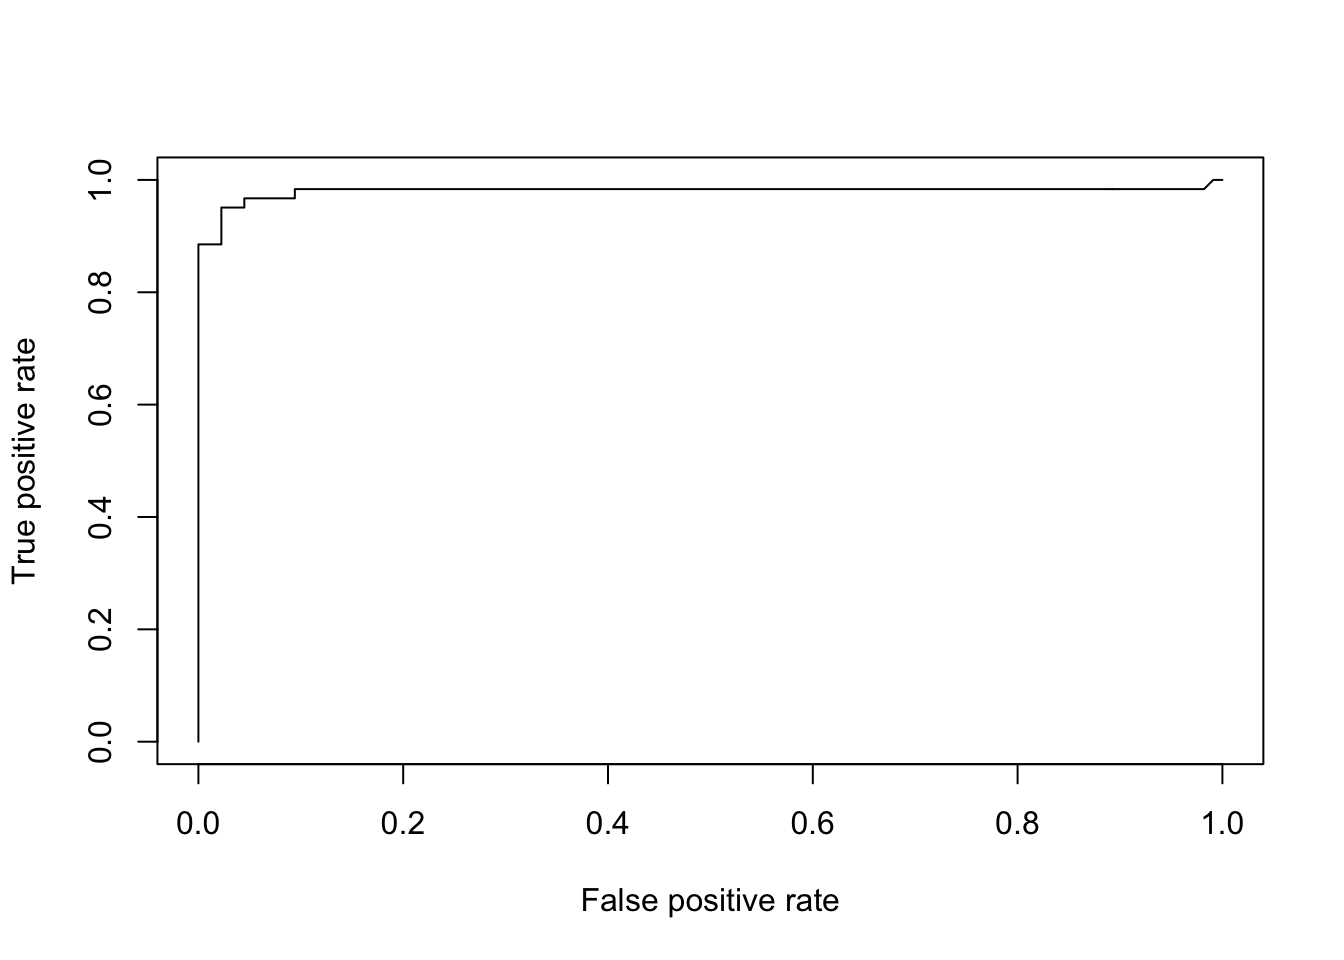
\includegraphics[width=0.45\textwidth]{results/post-update/memleak/boost-roc}
  }
  \caption[Post-Update, Memory Leak Using New Model Performance]{Performance of
  the boosting prediction method trained on failure data created after the
  software update obtained by consuming all available memory until target
  application fails.}
  \label{fig:memLeakPostUpdateBoostingPerf}
\end{figure*}
}

\newcommand{\figDPLGConceptDiagram}[1]{\begin{figure}
  \centering 
  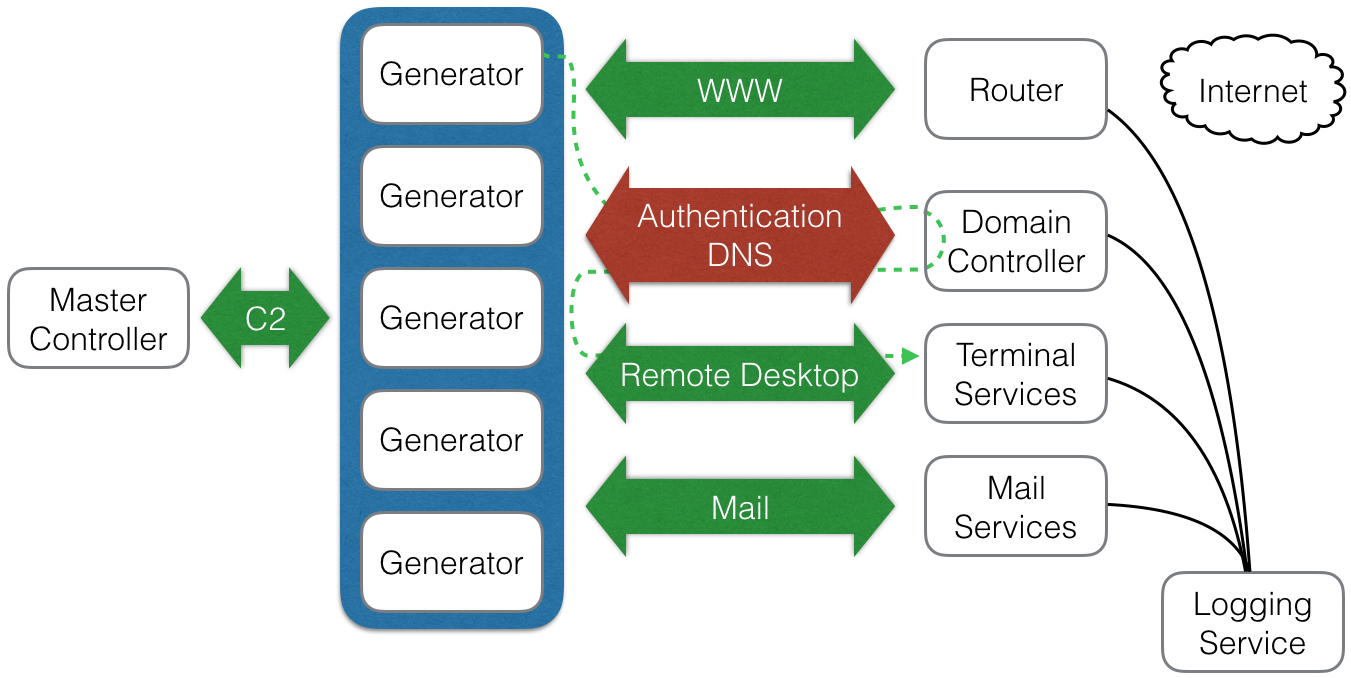
\includegraphics[width=#1]{DPLG/dplgConceptDiagram}
  \caption[Concept Diagram]{How each type of traffic that is generated is
  routed.  Log events are offloaded to logging service for further analysis.}
  \label{fig:conceptDiagram} 
  \end{figure}
}

\newcommand{\figDPLGAllModsClientMetrics}[1]{\begin{figure}
  \centering
  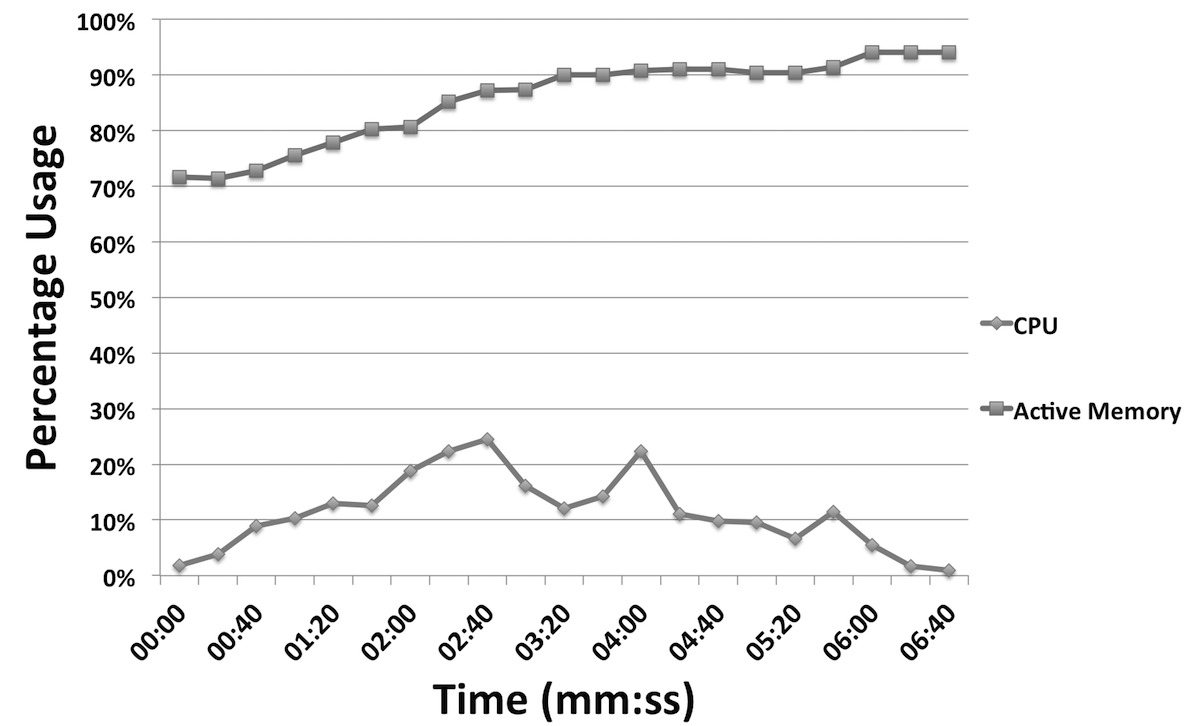
\includegraphics[width=#1]{DPLG/allModsClientMetrics}
  \caption[Test 2:  Client Metrics]{Client CPU and memory utilization during
  the second test.} \label{fig:allModsClientMetrics}
  \end{figure}
}


\newcommand{\tabFaults}{
\begin{table}[htbp]
  \centering
  \caption{Table of Faults Injected~\cite{gswfit}.}\label{tab:faults}
\begin{tabular}{ | c | l | c | } 
\hline
	\textbf{Type}  & \textbf{Description}  & \textbf{ODC Classes}  \\ \hline \hline
	MIFS  & Missing "If (cond) \{ statement(s) \}"  & Algorithm  \\ \hline
	MFC  & Missing function call  & Algorithm  \\ \hline
	MLAC  & Missing "AND EXPR" in expression used as branch & Checking  \\ \hline
	MLPC  & Missing small and localized part of the algorithm  & Algorithm  \\ \hline
	WVAV  & Wrong value assigned to a value  & Assignment  \\ \hline
	MVI  & Missing variable initialization  & Assignment  \\ \hline
	MVAV  & Missing variable assignment using a value  & Assignment  \\ \hline
	WPFV  & Wrong variable used in parameter of function call  & Interface  \\ \hline
\end{tabular}
\end{table}
}

\newcommand{\tabTranslationThirtyTwo}{
\begin{table}[htbp]
  \centering
  \caption{Funtion Entry/Exit Patterns
  (IA32)~\cite{gswfit}.}\label{tab:translationThirtyTwo}
\begin{tabular}{ | l | l | l | l | }
\hline
	\multicolumn{2}{|c|}{\textbf{Module Entry Point}}& 
  \multicolumn{2}{c|}{\textbf{Module Exit Point}} \\ \hline

	\textbf{Instruction Sequence} & \textbf{Explanation} &
  \textbf{Instruction Sequence} & \textbf{Explanation} \\ \hline \hline

	push ebp & stack frame & move esp,ebp & stack frame \\ \hline
	mov ebp, esp & setup & pop ebp & cleanup \\ \hline
	sub esp, \emph{immed} &  & ret &  \\ \hline
\end{tabular}
\end{table}
}

\newcommand{\tabTranslationSixtyFour}{
\begin{table}[htbp]
  \centering
  \caption{Funtion Entry/Exit Patterns
  (x86-64)~\cite{gswfit}.}\label{tab:translationSixtyFour}
\begin{tabular}{ | l | l | l | l | }
\hline
	\multicolumn{2}{|c|}{\textbf{Module Entry Point}}& 
  \multicolumn{2}{c|}{\textbf{Module Exit Point}} \\ \hline

	\textbf{Instruction Sequence} & \textbf{Explanation} & 
  \textbf{Instruction Sequence} & \textbf{Explanation} \\ \hline \hline

	push rbp & stack frame & add rsp, \emph{immed} & stack frame \\ \hline
	sub rsp, \emph{immed} &  & pop rbp & cleanup \\ \hline
	mov rbp, rdx & setup & ret &  \\ \hline
\end{tabular}
\end{table}
}

\newcommand{\tabHypervisorOne}{
\begin{table}[htbp]
  \centering
  \caption{Hypervisor 1 Configuration (Sandbox/Target).} \label{tab:hyp1}
  \begin{tabular}{ | c | l | l | c | l |}
    \hline
    Qty. & Role   & Operating System    & CPU / Mem. \\ \hline\hline
    1    & DC     & Win. Server 2008 R2 & 2 / 2 GB   \\ \hline
    5    & Client & Win. 7              & 1 / 512 MB \\ 
    \hline
  \end{tabular}
\end{table}
}


\newcommand{\tabHypervisorTwo}{
\begin{table}[htbp]
  \centering
  \caption{Hypervisor 2 Configuration (Controller).} \label{tab:hyp2}
  \begin{tabular}{ | c | l | l | c | l |}
    \hline
    Qty. & Role & Operating System    & CPU / Mem. \\ \hline\hline
    1    & RDP  & Win. Server 2008 R2 & 1 / 4 GB   \\ \hline
    1    & Log  & Ubuntu 14.04 LTS    & 1 / 1 GB   \\ 
    \hline
  \end{tabular}
\end{table}
}

\newcommand{\tabMessage}{
\begin{table}[!ht] \centering
  \caption{Typical authentication message sent as keys that correspond to the
  values as designated in the \emph{Snare} protocol for MSWinEventLog used by
  the SolarWinds syslog agent.} \label{tab:message}
  \begin{tabular}{ | l | l | }
    \hline
      Key                 & Value                               \\ \hline\hline
      HostName            & dc.afnet.com                        \\ \hline
      Criticality         & 5                                   \\ \hline
      EventLogSource      & Security                            \\ \hline
      Counter             & 3                                   \\ \hline
      SubmitTime          & Sun May 08 14:31:50 2016            \\ \hline
      EventID             & 4672                                \\ \hline
      SourceName          & Microsoft-Windows-Security-Auditing \\ \hline
      UserName            & N/A                                 \\ \hline
      SIDType             & Audit Success                       \\ \hline
      EventLogType        & dc.afnet.com                        \\ \hline
      ComputerName        & 12548                               \\ \hline
      CategoryString      & Special privileges assigned to\dots \\ \hline
      ExtendedDataString  & Security ID:  S-1-5-21-2379403\dots \\ 
    \hline
  \end{tabular}
\end{table}
}

\newcommand{\tabSlidingWindow}{
\begin{table}[!ht] \centering
  \caption{Sample time window after message translation.} \label{tab:window}
  \begin{tabular}{ | l | l | }
    \hline
      Key                         & Value \\ \hline\hline
      FailureWindow               & 0     \\ \hline
      NumObservations             & 2     \\ \hline
      Criticality: 6              & 2     \\ \hline
      Criticality: 2              & 0     \\ \hline
      Criticality: 4              & 0     \\ \hline
      EventLogSource: Application & 1     \\ \hline
      EventLogSource: System      & 1     \\ 
    \hline
  \end{tabular}
\end{table}
}

\newcommand{\tabMemLeakPreUpdateSVMStats}{
\begin{table}[!t] \centering
  \caption[Pre-Update, Memory Leak, SVM Statistics]{Classification statistics
  on test data created before software updates.}
  \label{tab:memLeakPreUpdateSVMStats}
  \begin{tabular}{ | l | l | }
    \hline
      Statistic           & Value  \\ \hline\hline
      True Positive Rate  & 0.8525 \\ \hline
      False Positive Rate & 0.0098 \\ \hline
      Accuracy            & 0.9777 \\ \hline
      Precision           & 0.8966 \\ \hline
      Recall              & 0.8525 \\ \hline
      F-Measure           & 0.8739 \\
    \hline
  \end{tabular}
\end{table}
}
%%%%%%%%%%%%%%%%%%%%%%%%%%%%%%%%%%%%%%%%%%%%%%%%%%%%%%%%%%%%%%%%%%%%%%%%%%%%%%%
%%%%   SVM   %%%%
% Pre-Update
\newcommand{\tabMemLeakPreUpdateSVMConfusionMatrix}{
  \begin{table}[!ht]
    \centering
    \caption[Pre-Update, Memory Leak, SVM Confusion Matrix]{Confusion matrix on
    test data created before software updates on threshold with highest
    F-Measure (0.8739) using SVM.}
    \label{tab:memLeakPreUpdateSVMConfusionMatrix}
    \begin{tabular}{llll}
                                                               &                                       & \multicolumn{2}{c}{\textbf{Actual}}                                        \\ \cline{3-4} 
                                                               & \multicolumn{1}{l|}{}                 & \multicolumn{1}{l|}{\textbf{Fail}} & \multicolumn{1}{l|}{\textbf{No-Fail}} \\ \cline{2-4} 
      \multicolumn{1}{c|}{\multirow{2}{*}{\textbf{Predicted}}} & \multicolumn{1}{l|}{\textbf{Fail}}    & \multicolumn{1}{l|}{52}            & \multicolumn{1}{l|}{6}                \\ \cline{2-4} 
      \multicolumn{1}{c|}{}                                    & \multicolumn{1}{l|}{\textbf{No-Fail}} & \multicolumn{1}{l|}{9}             & \multicolumn{1}{l|}{607}              \\ \cline{2-4} 
    \end{tabular}
  \end{table}
}

% Post-Update (old model)

% Post-Update New Model

%%%%   BOOSTING   %%%%
% Pre-Update
\newcommand{\tabMemLeakPreUpdateBoostingConfusionMatrix}{
  \begin{table}[!ht]
    \centering
    \caption[Pre-Update, Memory Leak, Boosting Confusion Matrix]{Confusion
    matrix on test data created before software updates on threshold with
    highest F-Measure (0.9917) using boosting.}
    \label{tab:memLeakPreUpdateBoostingConfusionMatrix}
    \begin{tabular}{llll}
                                                               &                                       & \multicolumn{2}{c}{\textbf{Actual}}                                        \\ \cline{3-4} 
                                                               & \multicolumn{1}{l|}{}                 & \multicolumn{1}{l|}{\textbf{Fail}} & \multicolumn{1}{l|}{\textbf{No-Fail}} \\ \cline{2-4} 
      \multicolumn{1}{c|}{\multirow{2}{*}{\textbf{Predicted}}} & \multicolumn{1}{l|}{\textbf{Fail}}    & \multicolumn{1}{l|}{60}            & \multicolumn{1}{l|}{0}                \\ \cline{2-4} 
      \multicolumn{1}{c|}{}                                    & \multicolumn{1}{l|}{\textbf{No-Fail}} & \multicolumn{1}{l|}{1}             & \multicolumn{1}{l|}{412}              \\ \cline{2-4} 
    \end{tabular}
  \end{table}
}

% Post-Update (old model)
\newcommand{\tabMemLeakPostUpdateBoostingSameModelConfusionMatrix}{
  \begin{table}[!ht]
    \centering
    \caption[Post-Update, Memory Leak, Same Model, Confusion
    Matrix]{Post-update failure data confusion matrix on threshold with highest
    F-Measure (0.4691) using model trained on failure data generated before
    software update.}
    \label{tab:memLeakPostUpdateBoostingSameModelConfusionMatrix}
    \begin{tabular}{llll}
                                                               &                                       & \multicolumn{2}{c}{\textbf{Actual}}                                        \\ \cline{3-4} 
                                                               & \multicolumn{1}{l|}{}                 & \multicolumn{1}{l|}{\textbf{Fail}} & \multicolumn{1}{l|}{\textbf{No-Fail}} \\ \cline{2-4} 
      \multicolumn{1}{c|}{\multirow{2}{*}{\textbf{Predicted}}} & \multicolumn{1}{l|}{\textbf{Fail}}    & \multicolumn{1}{l|}{19}            & \multicolumn{1}{l|}{1}                \\ \cline{2-4} 
      \multicolumn{1}{c|}{}                                    & \multicolumn{1}{l|}{\textbf{No-Fail}} & \multicolumn{1}{l|}{42}            & \multicolumn{1}{l|}{222}              \\ \cline{2-4} 
    \end{tabular}
  \end{table}
}

% Post-Update New Model
\newcommand{\tabMemLeakPostUpdateBoostingConfusionMatrix}{
  \begin{table}[!ht]
    \centering
    \caption[Post-Update, Memory Leak, New Model, Confusion
    Matrix]{Post-update failure data confusion matrix on threshold with highest
    F-Measure (0.9355) using model trained on failure data generated after
    software update.}
    \label{tab:memLeakPostUpdateBoostingConfusionMatrix}
    \begin{tabular}{llll}
                                                               &                                       & \multicolumn{2}{c}{\textbf{Actual}}                                        \\ \cline{3-4} 
                                                               & \multicolumn{1}{l|}{}                 & \multicolumn{1}{l|}{\textbf{Fail}} & \multicolumn{1}{l|}{\textbf{No-Fail}} \\ \cline{2-4} 
      \multicolumn{1}{c|}{\multirow{2}{*}{\textbf{Predicted}}} & \multicolumn{1}{l|}{\textbf{Fail}}    & \multicolumn{1}{l|}{58}            & \multicolumn{1}{l|}{5}                \\ \cline{2-4} 
      \multicolumn{1}{c|}{}                                    & \multicolumn{1}{l|}{\textbf{No-Fail}} & \multicolumn{1}{l|}{3}             & \multicolumn{1}{l|}{218}              \\ \cline{2-4} 
    \end{tabular}
  \end{table}
}

%%%%%%%%%%%%%%%%%%%%%%%%%%%%%%%%%%%%%%%%%%%%%%%%%%%%%%%%%%%%%%%%%%%%%%%%%%%%%%%
\newcommand{\tabModelSelection}{
\begin{table*}[!t]
  \centering
  \caption{Cross-validation runs on training data for model selection and
  resulting classification accuracy.}
  \label{tab:model:selection}
  \begin{tabular}{cllllllllllll}
    \multicolumn{1}{l}{}                       & \multicolumn{12}{c}{{\ul \textbf{Amount of Training Data}}}                                                                                                                                                                                         \\ \cline{2-13} 
    \multicolumn{1}{l|}{{\ul \textbf{Window}}} & \multicolumn{4}{c}{One Failure}                                             & \multicolumn{4}{c}{Two Failures}                                                & \multicolumn{4}{c|}{Four Failures}                                              \\ \cline{2-13} 
    \multicolumn{1}{c|}{\multirow{2}{*}{30s}}  & \textbf{Linear:}  & 0.0557 & \textbf{Poly:}   & \multicolumn{1}{l|}{0.0523} & \textbf{Linear:}  & 0.0756 & \textbf{Poly:}   & \multicolumn{1}{l|}{0.0659} & \textbf{Linear:}  & 0.0733 & \textbf{Poly:}   & \multicolumn{1}{l|}{0.0547} \\
    \multicolumn{1}{c|}{}                      & \textbf{Sigmoid:} & 0.0626 & \textbf{Radial:} & \multicolumn{1}{l|}{0.0459} & \textbf{Sigmoid:} & 0.0591 & \textbf{Radial:} & \multicolumn{1}{l|}{0.0438} & \textbf{Sigmoid:} & 0.0794 & \textbf{Radial:} & \multicolumn{1}{l|}{0.0542} \\ \cline{2-13} 
    \multicolumn{1}{c|}{\multirow{2}{*}{60s}}  & \textbf{Linear:}  & 0.0628 & \textbf{Poly:}   & \multicolumn{1}{l|}{0.0662} & \textbf{Linear:}  & 0.0779 & \textbf{Poly:}   & \multicolumn{1}{l|}{0.064}  & \textbf{Linear:}  & 0.0791 & \textbf{Poly:}   & \multicolumn{1}{l|}{0.0779} \\
    \multicolumn{1}{c|}{}                      & \textbf{Sigmoid:} & 0.1084 & \textbf{Radial:} & \multicolumn{1}{l|}{0.0487} & \textbf{Sigmoid:} & 0.1328 & \textbf{Radial:} & \multicolumn{1}{l|}{0.071}  & \textbf{Sigmoid:} & 0.2159 & \textbf{Radial:} & \multicolumn{1}{l|}{0.0797} \\ \cline{2-13} 
    \multicolumn{1}{c|}{\multirow{2}{*}{90s}}  & \textbf{Linear:}  & 0.1272 & \textbf{Poly:}   & \multicolumn{1}{l|}{0.0897} & \textbf{Linear:}  & 0.1131 & \textbf{Poly:}   & \multicolumn{1}{l|}{0.0732} & \textbf{Linear:}  & 0.0826 & \textbf{Poly:}   & \multicolumn{1}{l|}{0.0543} \\
    \multicolumn{1}{c|}{}                      & \textbf{Sigmoid:} & 0.1792 & \textbf{Radial:} & \multicolumn{1}{l|}{0.0779} & \textbf{Sigmoid:} & 0.2684 & \textbf{Radial:} & \multicolumn{1}{l|}{0.0757} & \textbf{Sigmoid:} & 0.2404 & \textbf{Radial:} & \multicolumn{1}{l|}{0.0552} \\ \cline{2-13} 
    \multicolumn{1}{c|}{\multirow{2}{*}{120s}} & \textbf{Linear:}  & 0.132  & \textbf{Poly:}   & \multicolumn{1}{l|}{0.104}  & \textbf{Linear:}  & 0.1452 & \textbf{Poly:}   & \multicolumn{1}{l|}{0.0785} & \textbf{Linear:}  & 0.0998 & \textbf{Poly:}   & \multicolumn{1}{l|}{0.0705} \\
    \multicolumn{1}{c|}{}                      & \textbf{Sigmoid:} & 0.204  & \textbf{Radial:} & \multicolumn{1}{l|}{0.104}  & \textbf{Sigmoid:} & 0.2864 & \textbf{Radial:} & \multicolumn{1}{l|}{0.0585} & \textbf{Sigmoid:} & 0.3056 & \textbf{Radial:} & \multicolumn{1}{l|}{0.0792} \\ \cline{2-13} 
  \end{tabular}
\end{table*}
}

\makeglossaries
\newacronym{AFP}{AFP}{Adaptive Failure Prediction}
\newacronym{OFP}{OFP}{Online Failure Prediction}
\newacronym{CPU}{CPU}{Central Processing Unit}
\newacronym{G-SWFIT}{G-SWFIT}{Generic Software Fault Injection Technique}
\newacronym{W-SWFIT}{W-SWFIT}{Windows Software Fault Injection Tool}
\newacronym{CSCS}{CSCS}{Cyber Security and Control System}
\newacronym{NOS}{NOS}{Network Operation Squadrons}
\newacronym{DOD}{DOD}{Department of Defense}
\newacronym{GHSMM}{GHSMM}{Generalized Hidden Semi-Markov Model}
\newacronym{SVM}{SVM}{Support Vector Machine}
\newacronym{IP}{IP}{Internet Protocol}
\newacronym{CRISP-DM}{CRISP-DM}{Cross Industry Standard Process for Data Mining}
\newacronym{ROC}{ROC}{Receiver Operating Characteristic}
\newacronym{MS}{MS}{Microsoft}
\newacronym{AD}{AD}{Active Directory}
\newacronym{GB}{GB}{Gigabyte}
\newacronym{GHz}{GHz}{Gigahertz}
\newacronym{VM}{VM}{Virtual Machine}
\newacronym{PFM}{PFM}{Proactive Fault Management}
\newacronym{DC}{DC}{Domain Controller}
\newacronym{ASLR}{ASLR}{Address Space Layout Randomization}
\newacronym{DNS}{DNS}{Domain Name System}
\newacronym{D-PLG}{D-PLG}{Distributed PowerShell Load Generator}
\newacronym{RDP}{RDP}{Remote Desktop Protocol}
\newacronym{SQL}{SQL}{Structured Query Language}
\newacronym{API}{API}{Application Programming Interface}
\newacronym{TP}{TP}{True Positive}
\newacronym{FP}{FP}{False Positive}
\newacronym{TN}{TN}{True Negative}
\newacronym{FN}{FN}{False Negative}
\newacronym{FPR}{FPR}{False Positive Rate}
\newacronym{TPR}{TPR}{True Positive Rate}
\newacronym{NPV}{NPV}{Negative Predictive Value}
\newacronym{AUC}{AUC}{Area Under the Curve}
\newacronym{IIS}{IIS}{Internet Information Service}
\newacronym{ODC}{ODC}{Orthogonal Defect Classification}
\newacronym{ANN}{ANN}{Artificial Neural Network}
\newacronym{NN}{NN}{Neural Network}
\newacronym{RNN}{RNN}{Recurrent Neural Network}
\newacronym{LSTM}{LSTM}{Long Short-Term Memory}


\begin{document}

%\jvol{00} \jnum{00} \jyear{2014} \jmonth{January}

\title{Data Driven Device Failure Prediction}

\author{Paul Jordan$^{\rm a}$ \
        Gilbert Peterson$^{\rm a}$ \
        Michael Mendenhall$^{\rm a}$ \
        Alan Lin$^{\rm a}$ \
        Andrew Sellers$^{\rm b}$ \\\vspace{6pt} \
        $^{a}${\em{Air Force Institute of Technology, Dayton, OH, USA}}; \\
        $^{b}${\em{United States Air Force Academy, Colorado Springs, CO, USA}}}
  
\maketitle

\begin{abstract}
As society becomes more dependent upon computer systems to perform increasingly
critical tasks, ensuring that those systems do not fail becomes increasingly
important.  Many organizations depend heavily on desktop computers for
day-to-day operations. Unfortunately, the software that runs on these computers
is written by humans and, as such, is still subject to human error and
consequent failure. A natural solution is to use statistical machine learning
to predict failure. However, since failure is still a relatively rare event,
obtaining labelled training data to train these models is not a trivial task.
This work presents new simulated fault-inducing loads that extend the focus of
traditional fault injection techniques to predict failure in the Microsoft
enterprise authentication service and Apache web server. These new fault loads
were successful in creating failure conditions that were identifiable using
statistical learning methods, with fewer \hl{irrelevant} faults being created.


\begin{keywords}
online failure prediction; machine learning; fault injection; enterprise
architecture
\end{keywords}

\end{abstract}

As we become more dependent upon computers and they permeate their way into our
daily lives, we need to consider the risks associated.  Computer systems are
literally all around us.  Some of these computer systems play insignificant
roles in our lives while others may be responsible for sustaining our lives.
Unfortunately, the software that controls these systems is written by humans
and consequently subject to human error.  As a result, these systems are prone
to failure which in many cases may not be a big deal, but in others, could have
severe consequences.  Every day, critical infrastructure and Air Force missions
systems depend on the reliability of computer systems.  As a result, being able
to predict pending failue in computer systems can offer tremendous and
potentially life-saving applications in todays technologically advanced world.
While actually being able to accurately predict failure has unfortunately not
been proven possible, there has been an enormous amount of time and energy
spent over the past several decades attempting to make educated predictions
about the failure of machines through the use of sophisticated machine learning
algorithms.  Unfortunately, much of this work has gone unused.  

There a number of ways to reduce the number of errors produced by a piece of
software, but the software development life-cycle is shrinking and less time
and effort are being devoted to reducing errors before deployment.  This leaves
real-time error prevention or handling.  In recent years, it seems many of the
cloud based computing companies have attempted to solve problems caused by
machine failure by making all of their services massively redundant.  As
hardware becomes more affordable, this is an effective approach in many ways,
but ultimately is still not cost efficient.  In some cases, funds may not be
available to acheive this sort of redundancy.  Consequently, this research
focuses on a small piece of the general field of reliable computing: online
failure prediction (OFP).  OFP is the act of attempting to predict when
failures are likely so that they can be avoided.  A great deal of work has been
done in this field which we outline in Chapter~\ref{chapter2}, but much of it
has gone unimplemented due to the complex and manual task of training a
prediction model.  If the underlying system changes at all the efficacy of a
prediction model can be drastically reduced if not rendered completely useless
until it is retrained.  Furthermore, training requires access to labelled
training data.  Since failure is such a rare event, access to this type of
training data may not be possible.  

Irrera et al.~\cite{irrera2015} presented a potential solution in 2015 to
automate the process of dynamically generating failure data and using it to
train a predictor after an underlying system change.  They defined a framework
for implementing this process and called it the Adaptive Failure Prediction
(AFP) Framework.  This research explores an implementation of that framework.
More specifically, we present our results after implementing the AFP using a
Microsoft Windows Server domain controller.  We then apply successive software
updates until the model we have selected becomes useless and allow the
framework to re-train our predictor.

\section{Problem Statement}
Predicting and alerting on impending network service failures currently uses
thresholds and rules on discrete items in enterprise system logs.  For example,
if the central processing unit (CPU) and memory usage on a device exceeds 90\%,
then an alert may be issued.  This approach works, but only for certain types
of failures and in order to minimize the false positives, it only makes
recommendations minutes before a failure, or when the system is in an already
degraded performance mode.  To maintain network resilience, the operational
organizations responsible for communications support desperately need some
means of gaining lead-time before a service failure occurs.  

Preceding a service failure event, multiple indicators spread disparate
sources, perhaps over a long period of time, may appear in system logs.  The
log entries of interest are also quite rare compared with normal operations.
Because of these constraints, identifying failure indicators can be nearly
impossible for humans to perform.  Further, in most cases, restoring service is
more important than identifying the indicators that may or may not have
existed.  

Failure prediction can be approached in many ways. Arguably the simplest
approach is to use everyday statistical analysis to, for example, determine the
mean time between failures of specific components. The analysis of all
components making up a system can be aggregated to make predictions about that
system using a set of statistics-based or business-relevant rules.
Unfortunately, the complexity of modern architectures has outpaced such
off-line statistical-based analysis, which has driven the advancement of OFP.
OFP differs from other means of failure prediction in that it focuses on
classifying the current running state of a machine as either failure prone or
not, or in such a way that it describes the confidence in how failure prone a
system is at present~\cite{salfnerSurvey}.

Unfortunately, in recent years much of the work in OFP has gone unused due to
the dramatic decrease in cost and complexity involved in building
hardware-based redundant systems.  Furthermore, in most cases OFP implements
machine learning algorithms that require manual re-training after underlying
system changes.  More troubling is that these system changes are becoming more
frequent as the software development life cycle moves toward a more continuous
integration model.  To help solve these challenges, the framework presented
in~\cite{irrera2015} uses simulated faults to automatically re-train a
prediction algorithm to make implementing OFP approaches easier.  We propose to
expand the work in~\cite{irrera2015} to capture developments since its writing
and generalize it so it works for a broader class of devices.

\section{Impact of Research}
Every day, many of the Air Force's critical missions depend on our computer
infrastructure.  An essential piece of this infrastructure is the
authentication mechanisms that protect our sensitive information.
Unfortunately, the software at the core of this infrastructure is written and
maintained by humans and thus susceptible human error.  This research will
enable the Air Force and many others that use the Microsoft Enterprise
Infrastructure to accurately predict pending service outages thereby providing
lead-time in order to avoid those outages.  The result is cost savings in
personnel, equipment, but isn't limited to cost savings.  It is difficult to
quantify the risk of mission failure due to network service outage.

\section{Assumptions and Limitations}
As previously stated, it has not been proven possible to accurately predict
future events without a priori knowledge.  As a result, this research depends
on the fact that there are indicators of failure present and available to us
with enough lead-time to accurately make decisions and take mitigation action
should failure be predicted based on these indicators.  This research presents
a method of predicting failure, but this method is completely useless at
predicting \emph{act of God} events.  Further, this method is capable of
predicting failure based on software failures and cannot provide any useful
information about malicious attacks against the target software.

\section{Expected Results of Research}
Because a prediction method is not presently deployed on any Air Force network,
any level of dependable prediction will be better than what is currently
available.  This research will attempt to show that after an underlying system
change, this method of predicting failure will be capable of automatically
training a more effective prediction algorithm so that this technique can be
implemented on an Air Force network with little to no impact on manpower.
Consequently, we expect that this research will inform decision makers and
allow them to implement this technique in a production environment.

Specifically, we believe the technique presented in this research could most
effectively be implemented and used by the Cyber Security and Control System
(CSCS) weapon system employed at the 561st and 83d Network Operation Squadrons
(NOS) and their associated detachments to reduce the number of network service
outages, increasing uptime, leading to improved mission effectiveness in both
the support and operational domains.  Further, we believe this technique
general enough to be employed outside of the Air Force to increase mission
effectiveness across the Department of Defense (DOD).  External to the DOD,
this research further generalizes an approach that could be used to help
increase availability of nearly any computer system.
        % 1 Page
\section{Overview of \ac{OFP}} \label{chapter2}
Traditionally, failure is predicted using statistical information about past
failures offline before a system is implemented.  Unfortunately, given the
complexity of modern computer systems and the infinite number of ways in which
they can be configured, this sort of offline analysis is not helpful.  \ac{OFP}
is the act of evaluating a running system in real time to make a prediction
about what the future state will be.

This chapter reviews current research regarding \ac{OFP} and its many
approaches to build a foundation for this research.  Further, the taxonomy of
approaches developed by Salfner, et al.~\cite{salfnerSurvey}, is updated by
classifying approaches since its publication and creating a new sub-category.
The rest of this chapter is organized as follows.  In Section~\ref{background},
a brief background on the topic of \ac{OFP} is given including definitions,
terminology, and measures of performance used by the community.  In
Section~\ref{approaches}, the approaches relevant to this research are
presented.  This chapter then concludes with a brief summary.

\subsection{Background} \label{background}
In 2010, Salfner, et al.~\cite{salfnerSurvey} published a survey paper that
provides a comprehensive summary of the state of the art on the topic of
\ac{OFP}.  In addition to the review of the literature up to the point of
publication, they provide a summary of definitions and measures of performance
commonly used in the community for couching the \ac{OFP} discussion.  The
remainder of this section reviews those definitions to build a foundation for
the rest of this work.

\subsubsection{Definitions} \label{definitions}
\paragraph{\ac{PFM}} \label{pfm}
Salfner, et al.~\cite{salfnerSurvey} define \ac{PFM} as the process by which
faults are handled in a proactive way, analogous with \emph{fault tolerance}
and basically consisting of four steps: \ac{OFP}, diagnosis, action scheduling,
and action execution as shown in Figure~\ref{fig:proactiveFaultManagement}.
The final three stages of \ac{PFM} define how much lead time is required to
avoid a failure when predicted during \ac{OFP}.  \emph{Lead time} is defined as
the time between when failure is predicted and when that failure will occur.
Lead time is one of the most critical elements of a failure prediction
approach.

\figproactiveFaultManagement{0.8\textwidth}

\ac{OFP} is defined as the first step in \ac{PFM} shown in
Figure~\ref{fig:proactiveFaultManagement}.  \ac{OFP} is the act of analyzing
the running state of a system in order to predict failure in that system. Once
failure has been predicted, a fault tolerant system must determine what will
cause the failure.  This stage is called the \emph{diagnosis} stage or
``root-cause analysis'' stage.  During the \emph{diagnosis} stage, analysis
must be conducted to identify possible remediation actions.  After it is
determined what will cause a failure, a fault tolerant system must schedule a
remediation action that is either performed by an operator or done
automatically.  This stage is known as the \emph{action scheduling} stage and
normally takes as input the cost of performing an action, confidence in
prediction, effectiveness/complexity of remedy action and makes a decision
about what action to perform based on that input.  In some cases a remedy
action can be so simple that even if the confidence in the prediction is low,
the action can still be performed with little impact on the overall system and
its users.  A thorough analysis of the trade-off between cost of avoidance and
confidence in prediction and the associated benefits is described
in~\cite{candea2004microreboot}.  Finally, in order to avoid failure, a system
must execute the scheduled remediation action or let an operator know which
actions can be taken in a stage called \emph{action execution}.

\paragraph{Faults, Errors, Symptoms, and Failures}
This research uses the definitions from~\cite{avivzienis2004basic} as
interpreted and extended in~\cite{salfnerSurvey} for the following terms:
failure; error (detected versus undetected); fault; and symptom.

\emph{Failure} is an event that occurs when the delivered service deviates from
correct service.  In other words, things can go wrong internally; as long as
the output of a system is what is expected, failure has not occurred.  

An \emph{error} is the part of the total state of the system that may lead to
its subsequent service failure.  \emph{Errors} are characterized as the point
when things go wrong~\cite{salfnerSurvey}.  Fault tolerant systems can handle
errors without necessarily evolving into failure.  There are two kinds of
errors.  First, a \emph{detected error} is an error that is reported to a
logging service.  In other words, if it can be seen in a log then it is a
detected error.  Second, \emph{undetected errors} are errors that have not been
identified by an error detector.  Undetected errors are things like memory
leaks.  The error exists, but as long as there is usable memory, it is not
likely to be reported to a logging service.  Once the system runs out of usable
memory, undetected errors will likely appear in logs and become a detected
errors.  A \emph{fault} is the hypothesized root cause of an error.  Faults can
remain dormant for some time before manifesting themselves and causing an
incorrect system state.  In the memory leak example, the missing \emph{free}
statement in the source code would be the fault.  

A \emph{symptom} is an out-of-norm behavior of a system's parameters caused by
errors, whether detected or undetected.  In the memory leak example, a possible
symptom of the error might be delayed response times due to sluggish
performance of the overall system.

\figfailureFlowDiagram{\textwidth}

Figure~\ref{fig:failureFlowDiagram} illustrates how a software fault can evolve
into a failure.  Faults, errors, symptoms, and failures can be further
categorized by how they are detected also shown in
Figure~\ref{fig:failureFlowDiagram}.  Salfner, et al.~\cite{salfnerSurvey}
introduces a taxonomy of \ac{OFP} approaches and classifies failure prediction
approaches by the stage at which a fault is detected as it evolves into a
failure: auditing, reporting, monitoring, and tracking.  Testing is left out
because it does not help detect faults in an online sense.  

\figonlinePrediction{0.8\textwidth}

Figure~\ref{fig:onlinePrediction} demonstrates the timeline associated with
\ac{OFP}.  The parameters used by the community to define a predictor are as
follows:
\begin{itemize}
	\item{Present Time: $t$}
  \item{Lead Time: $\Delta t_{l}$, is the total time at which a predictor makes
  an assessment about the current state.}
  \item{Data Window: $\Delta t_{d}$, represents the time from which data is
  used for a predictor uses to make its assessment.}
  \item{Minimal Warning Time: $\Delta t_{w}$, is the amount of time required to
  avoid a failure if one is predicted.}
  \item{Prediction Period: $\Delta t_{p}$, is the time for which a prediction
  is valid.  As $\Delta t_{p} \rightarrow \infty$, the accuracy of the
  predictor approaches 100\% because every system will eventually fail.  As
  this happens, the usefulness of a predictor is diminished.}
\end{itemize}

As the above parameters are adjusted, predictors can become more or less
useful.  For example, it is clear that as a predictor looks further into the
future potentially increasing \emph{lead time}, confidence in its prediction is
likely to be reduced.  On the other hand, if \emph{lead time} is too small,
there will likely not be enough time to effectively take remediation action.
In general, \ac{OFP} approaches seek to find a balance between the parameters,
within an acceptable bound depending on application, to achieve the best
possible performance.

\subsection{Approaches to \ac{OFP}} \label{approaches}
\subsubsection{\ac{OFP} Taxonomy}
The taxonomy by Salfner, et al.~\cite{salfnerSurvey} classifies many of the
\ac{OFP} approaches in the literature into four major categories.  These four
major categories are defined by the four techniques used to detect faults in
real-time: auditing, monitoring, reporting, and tracking as illustrated in
Figure~\ref{fig:failureFlowDiagram}.  The taxonomy is shown in
Figure~\ref{fig:OFPTaxonomy}.

\figOFPTaxonomy{0.8\textwidth}

Since this research focusses on real-time \emph{data-driven} device failure
prediction approaches, our focus is on the \emph{reporting} category of
Salfner's taxonomy.  The \emph{reporting} category organizes failure prediction
techniques that attempt to classify a state as failure prone based on reported
errors.  This is different from prediction methods that rely on observing the
current state of a machine such as auditing and monitoring.  As pointed out by
Salfner, et al.~\cite{salfnerSurvey}, in general these methods have difficulty
distinguishing a system under peak load and one that may be about to fail.

The reporting category of the taxonomy is further organized into five
sub-categories: rule-based systems; co-occurrence; pattern recognition;
statistical tests; and classifiers.

\emph{Rule-Based Systems} attempt to classify a system as being failure-prone
or not based a set of conditions met by reported errors.  Since modern systems
are far too complex to build a set of conditions manually, these approaches
seek to find automated ways of identifying these conditions in training data.
\emph{Co-occurrence} predictors generate failure predictions based on the
reported errors that occur either spatially or temporally close together.
\emph{Pattern Recognition} predictors attempt to classify patterns of reported
errors as failure prone.  \emph{Statistical Tests} attempt to classify a system
as failure-prone based on statistical analysis of historical data.  For
example, if a system is generating a much larger volume of error reports than
it typically does, it may be a sign of pending failure.  \emph{Classifiers}
assign labels to given sets of error reports in training data and then make
failure predictions based on observed labels in real-time data.  

This research focusses on pattern recognition OFP approaches, which are shown
in Figure~\ref{fig:patternRecognition}.  Strategies employed in the other
sub-categories are closely related and thus are also explored in this research.

\figpatternRecognition{\textwidth}

\subsubsection{Data-Driven \ac{OFP}}
% The survey published by Salfner et al. covered approaches in every sub-category
% of the \emph{reporting} category.  Since the publication of the survey, the
% majority of approaches published have been in two of the subcategories,
% \emph{pattern recognition} and \emph{classifiers}.  We therefore only cover
% the approaches in those sub-categories of the reporting category here.  We
% found some of the approaches published since Salfner's survey to be difficult
% to classify because they employ aspects of the other sub-categories in the
% \emph{reporting} category.  More specifically, many of the modern techniques
% seem to be a blend between the two sub-categories \emph{pattern recognition}
% and \emph{classifiers}.  We believe these categories have been blended
% because these approaches seem to follow general human intuition when looking
% for software failures.  In other words, we have found that cyber operators
% tend to look for patterns in reported errors and then classify a situation
% based on those patterns.  We therefore categorize these approaches as
% \emph{hybrid} approaches.

\paragraph{Pattern Recognition}
Salfner, et al.~\cite{salfner2006} proposed an approach to predicting failures
by learning patterns of similar events using a semi-Markov chain model.
The model learned patterns of error reports that led to failure by mapping the
reported errors to the states in the Markov chain and predicted the probability
of the transition to a failure-prone state.  They tested the model using
performance failures of a telecommunication system and reported a precision of
0.8, recall of 0.923, and an F-measure of 0.8571, which drastically
outperformed the models to which it was compared.

Given the results, the semi-Markov Chain model is compelling however, it
depends on the sequence of reported errors to remain constant in order to be
effective.  Today, most software is multi-threaded or distributed so there is
no guarantee that the sequence of reported errors will remain constant.
Further, the authors reported that this approach did not scale well as the
complexity of the reported errors grew.

In 2007, Salfner, et al. extended their previous work in~\cite{salfner2006}
using semi-Markov models~\cite{salfner2007}.  They generalized the Hidden
Semi-Markov process for a continuous-time model and called it the \ac{GHSMM}.
By making this generalization, the model was able to effectively predict the
sequence of similar events (or in this case, errors) in the continuous time
domain.  The authors then tested the model and training algorithm using
telecommunication performance failure data and compared it to three other
approaches.  While this \ac{GHSMM} model did not perform as well as their
previous work, it did outperform the models to which it was compared and more
importantly did not depend on the sequence of reported errors.  In other words,
this new \ac{GHSMM} model predicted failure for permutations of a known
failure-prone sequence making it more suited for a distributed or parallel
system.

The \ac{GHSMM} approach has been well received by the community, although
appears to be limited in use to a single system.  Unfortunately, this approach
as well as its predecessor, does not scale well and does not adapt to changes
to the underlying system without retraining.

\paragraph{Classifiers}
Domeniconi, et al.~\cite{domeniconi2002} published a technique that used
\ac{SVM} to classify the present state as either failure prone or not based on
a window of error reports as an input vector.  As Salfner points out
in~\cite{salfnerSurvey}, this \ac{SVM} approach would not be useful without
some sort of transformation of the input vector since the exact same sequence
of error messages, rotated by one message, would not be classified as similar.
To solve this permutation challenge, the authors in~\cite{domeniconi2002} used
singular value decomposition to isolate the sequence of error reports that led
to a failure.

This \ac{SVM} approach used training data from a production computer
environment with 750 hosts over a period of 30 days.  The types of failures the
system was trying to detect was the inability to route to a web-page and an
arbitrary node being down.  Many approaches involving \ac{SVM}s have been
explored since and seem to be popular in the community~\cite{fronza2013,
fulp2008, murray2005, domeniconi2002, irrera2015}.

\paragraph{Hybrid Approaches}
\emph{Fujitsu Labs} has published several papers on an approach for predicting
failure in a cloud-computing
environment~\cite{sonoda2012,watanabe2012,watanabe2014}.  Watanabe, et
al.~\cite{watanabe2012, watanabe2014} report on findings after applying a
Bayesian learning approach to detect patterns in similar log messages.  Their
approach abstracts the log messages by breaking them down into single words and
categorizing them based on the number of identical words between multiple
messages.  This hybrid approach removes the details from the messages, like
node identifier, and \ac{IP} address while retaining meaning of the log
message.

Watanabe et al.'s~\cite{watanabe2014} hybrid approach attempts to solve the
problem of underlying system changes by learning new patterns of messages in
real-time.  As new messages come in, the model actively updates the probability
of failure by Bayesian inference based on the number of messages of a certain
type that have occurred within a certain time window.  The authors claim that
their approach solves three problems: 1)  The model is not dependent upon a
certain lexicon used to report errors to handle different messages from
different vendors; 2) The model does not take into account the order of
messages necessarily so in a cloud environment where messages may arrive in
different orders, the model is still effective; and 3)  The model actively
retrains itself so manual re-training does not need to occur after system
updates.  The model was then tested in a cloud environment over a ninety day
period.  The authors reported a precision of 0.8 and a recall of 0.9, resulting
in an F-measure of 0.847.  

Fronza, et al.~\cite{fronza2013} introduced a pattern-recognition/classifier
hybrid approach that used an \ac{SVM} to detect patterns in log messages that
would lead to failure.  The authors used random indexing to solve the problem
previously discussed of \ac{SVM}s failing to classify two sequences as similar
if they are offset by one error report.  The authors report that their
predictor was able to almost perfectly detect non-failure conditions but was
poor at identifying failures.  The authors then weighted the \ac{SVM}s to
account for this discrepancy by assigning a larger penalty for false negatives
than false positives and had better results.

\subsubsection{Industry Approaches to \ac{OFP}} \label{industry}
Because hardware has become so easy to acquire, industry has sought to avoid
the problem of software failure by implementing massive redundancy in their
systems.  The work in~\cite{irrera2015,watanabe2014} attributes the problem
avoidance to the fact that until recently, implementing and maintaining a
failure predictor was difficult.  As we decrease the length of the software
development life cycle, software updates are being published with increasing
frequency leading to rapid changes in underlying systems.  These changes can
often render a predictor useless without re-training, which is often a manual
and resource intensive process.

Redundancy is not without problems however.  Implementing redundant systems to
avoid the failure problem can be expensive and can add overhead and complexity
making a system more difficult to manage.

\subsubsection{\ac{AFP} Framework} \label{afp}
The \ac{AFP} framework by Irrera, et al.~\cite{irrera2015} shown in
Figure~\ref{fig:AFP}, presents a new approach to maintaining the efficacy of
failure predictors given underlying system changes.  The authors conducted a
case study implementing the framework using virtualization and fault injection
on a web server.  

\figAFP{0.8\textwidth}

The framework built upon past work by Irrera, et
al.~\cite{irrera2013,irrera2014} to generate failure data by injecting software
faults using a tool based on \ac{G-SWFIT}~\cite{gswfit} in a virtual
environment for comparing and automatically re-training predictors.  With the
introduction of the framework, Irrera, et al.~\cite{irrera2015} report results
of a case-study.  After implementing the \ac{AFP} framework using a web server
and an \ac{SVM} predictor, they report that their findings demonstrate their
framework is able to adapt to changes to an underlying system which would
normally render a predictor unusable.

In general, the use of simulated data is not well received by the community,
however the authors in~\cite{irrera2010,irrera2014} report evidence supporting
the claim that simulated failure data is representative of real failure data.
Further, the authors suggest that since systems are so frequently updated and
failures are in general rare events, real failure data is often not available.
Moreover, the literature shows that even if there is a certain type of failure
in training data and a predictor can detect and predict that type of error
accurately, it will still miss failures not present in the training data.  By
injecting the types of faults that one can expect, each failure type is
represented in the training data.

Irrera, et al.~\cite{irrera2015} reported good results and concluded that the
\ac{AFP} framework is an effective tool.  Unfortunately, the \ac{AFP} framework
is not a universal solution and requires significant work to be implemented on
a modern \ac{MS} Windows enterprise network.  Furthermore, the fault load
previously explored does not completely represent all possible
failures~\cite{kikuchi2014}.

\subsection{Summary} \label{summary}
This chapter covered the definitions, measures of performance, and approaches
that are relevant to this research as organized under the subsection of
\emph{reporting} within the \ac{OFP} field of study.  There has been a
tremendous amount of research surrounding the topic of \ac{OFP} and many
prediction approaches have been presented.  Unfortunately, these approaches do
not appear on modern operational systems and failures are still relatively
prevalent.  Recent approaches as covered here have sought to make predictors
more adaptive to the changes in underlying systems in an effort to make
implementing existing failure predictors easier.  In this work, we plan to
extend the \ac{AFP} framework and further generalize the
approach.  
 % 2-2.5 Pages
\section{Methodology} \label{chapter3}
The purpose of the \ac{AFP} framework is to automate the generation of
realistic labelled failure data for the purposes of automatically training a
failure prediction algorithm.  The framework breaks down into modules so that
it can be more easily adapted for different applications.  This chapter
presents three topics.  The first describes the process that the framework
executes in order to generate the labelled training data and train a failure
prediction algorithm.  The second describes each module of the extended
\ac{AFP} framework.  The final section details extensions to the \ac{AFP}
framework explored by this research.

This chapter outlines the implementation and extensions to the \ac{AFP}
framework~\cite{irrera2015} as well as an experiment that was conducted to
validate those extensions and further generalize the framework.  The \ac{AFP}
framework was originally tested on a single system running an operating system
that has been deprecated.  Consequently, the results from the case study
conducted using the \ac{AFP} framework are limited in utility and require
generalization to be useful to the general community.

\subsection{Failure Data Generation} \label{sec:generation}
This work extends the \ac{AFP} framework~\cite{irrera2015} by presenting
results after conducting another case study with an \ac{MS} Windows Server
acting as an \ac{AD} service with a more representative fault load as well as a
new implementation of the \ac{G-SWFIT} technique for the x86-64 architecture.
The case study was done using three new types of faults: third-party memory
leak, third-party \ac{CPU} hog, and process memory corruption.  For
completeness, the standard \ac{G-SWFIT} technique was also used.  Finally,
findings are reported after implementing this framework using two different
statistical machine learning techniques on reported errors (log messages):
boosted decision trees and the weighted \ac{SVM}.  The weighted \ac{SVM} was
used because of it performs well on imbalanced data and it is popular in the
\ac{OFP} community~\cite{salfnerSurvey}.  The boosted decision tree was used
because it is non-parametric, it is capable of classification, and it is
particularly suited for imbalanced data.  In both cases, feature reduction was
performed as is done by Fulp et al.~\cite{fulp2008}, on a sliding time window
as is done by Irrera, et al.~\cite{irrera2013a} and
Vaarandi~\cite{vaarandi2002}.

This section outlines the step-by-step procedure by which the extended \ac{AFP}
framework was evaluated to show how effective it is when used on Windows Server
deployments.  This is done by dividing the steps taken in the experiment into
the three major phases as defined in~\cite{irrera2015}: preparation phase,
execution phase, and training phase.

\subsubsection{Preparation Phase}
In this phase the \ac{AFP} framework is prepared to run for the first time as
described in~\cite{irrera2015}.  The \ac{CRISP-DM}~\cite{crispdm} should be
applied to this situation when evaluating how to best apply the \ac{AFP} for a
particular target.  For the purposes of this research, the focus was on the
\ac{MS} Windows Directory Services and predicting failure in those services.
To demonstrate the efficacy of the \ac{AFP}, a predictor was evaluated before
and after a significant software update.  As a result, the most critical
preparation made in evaluating this framework was to hold back all software
updates on the target system prior to the first run of the execution phase.
The performance of various prediction techniques were evaluated both before and
after the Windows Update application was allowed to run.  A complete list of
the updates installed is shown in Appendix~\ref{app:updates}.

This phase is essentially comprised of the manual act of implementing the
framework.  Each module of the implementation for this work is detailed in
Section~\ref{sec:implementation} and is therefore not discussed further here.  

\subsubsection{Execution Phase}
A general outline of this phase is shown in Figure~\ref{fig:ExecutionPhase}.
This phase is divided into three major steps: data collection and failure
prediction, event checking, and training/update as described in this section.

\figExecutionPhase{2.5in}

\paragraph{Data Collection and Failure Prediction}
In this phase, the system has a working predictor providing input to some sort
of decision system.  It should be noted here that this decision system does not
have to be automated.  The system in this phase makes failure predictions about
the current state based on the last run of the training phase.  This function
was not implemented in this research as it is application specific.  The output
of this process in this experiment was a warning message indicating a predicted
failure.

\paragraph{Event Checking}
Concurrent with the data collection and failure prediction sub-phase, the
\ac{AFP} framework continuously monitors events that may alter the underlying
system.  The output of each episode of this phase is a binary decision to
either begin the training phase, or not.  For this experiment, these events
were software updates and the training phase was manually triggered upon
completion of these updates.

\paragraph{Failure Predictor (Re-)Training and Update}
The purpose of this sub-phase is to initiate the training phase and compare its
results (a new predictor) with the currently employed predictor.  Should the
new predictor perform better, the old predictor is replaced by the new.  In
this experiment, this phase was accomplished manually.

\subsubsection{Training Phase}
The training phase is broken down into five major steps:  target replication,
data generation \& collection, dataset building, predictor training, and
analysis.  The general flow is shown in Figure~\ref{fig:TrainingPhase}.  Each
phase is outlined in the following sub-sections.

\figTrainingPhase{4in}

\paragraph{Target Replication}
During this phase a virtual clone of the target is made.  After the clone is
made, the fault injection and monitoring software is installed.  In this
experiment, the monitoring tool was the same as was already installed on the
production system so the extra step of installing the monitoring software was
unnecessary.

\paragraph{Data Generation \& Collection}
The purpose of this phase is to generate the data to train a new prediction
algorithm.  As a result, this sub-phase must be executed several times to
generate statistically meaningful datasets.  In this phase, the controller
triggers the cloned target startup.  Once startup is complete and the system
enters an idle state, the monitoring tool begins collecting data from the
target.  After monitoring has begun, the workload is started.  Once the
workload has entered a steady state, the fault load is started.  Finally, when
failure occurs, monitoring stops, the workload stops, and the system is
rebooted for the next run.  To generate golden data (or data with no failures
present to aid training), the first run omits the fault injection step.

The most critical part of this process is labelling the data when failure
occurs.  For the purposes of this experiment, failure was defined by the log
message ID $4625$: An account failed to log
on\footnote{\url{https://support.microsoft.com/en-us/kb/977519}}.  When this
occurred in conjunction with known valid credentials on an enabled account, the
preceding data window defined for the experiment was labelled as failure prone.
Additionally, the workload generator used in this research reported when
authentication failed and transmitted a syslog message to the controller.  

\paragraph{Dataset Building} \label{sec:dataset.building}
In this phase, the raw syslog messages are formatted and encoded to train the
prediction model.  The purpose of this phase is to prepare the raw messages to
be used as numeric inputs for the training phase.  Irrera, et
al.~\cite{irrera2015} loaded all event messages into a database for processing.
In this work, the events were initially stored in a flat file on the Ubuntu
machine by the syslog daemon.  The raw log messages appeared in a flat text
file as follows:

\begin{lstlisting}
May  8 14:31:52 dc.afnet.com MSWinEventLog 5 Security 3 Sun May 08 14:31:50 2016 4672 Microsoft-Windows-Security-Auditing  N/A Audit Success dc.afnet.com 12548 Special privileges assigned to new logon.  Subject:  Security ID:  S-1-5-21-2379403389-181978965-2953995107-500  Account Name:  Administrator  Account Domain:  AFNET  Logon ID:  0x9beb4e7a  Privileges:  SeSecurityPrivilege    SeBackupPrivilege    SeRestorePrivilege    SeTakeOwnershipPrivilege    SeDebugPrivilege    SeSystemEnvironmentPrivilege    SeLoadDriverPrivilege    SeImpersonatePrivilege    SeEnableDelegationPrivilege
\end{lstlisting}

The messages were formatted using the
\emph{Snare}\footnote{\url{http://wiki.rsyslog.com/index.php/Snare\_and\_rsyslog}}
MSWinEventLog format which is generally divided into several categories.  The
first is the time-stamp and host name of the sender prepended by the syslog
server daemon: \emph{May 8 14:31:52 dc.afnet.com}.  The remainder of the
message contains tab delimited values where the keys (and consequent features)
are shown in Table~\ref{tab:message}.  Of these features, Criticality,
EventLogSource, EventID, SourceName, and CategoryString were selected for
further encoding.

\tabMessage

The raw messages were then encoded.  First, the events were filtered by EventID
as is done by Fulp et al.~\cite{fulp2008} to reduce the noise generated by
successful login attempts.  Log messages with IDs shown in
Table~\ref{tab:messageIDs} were filtered from the input.  

Next, to encode the time dimension and reduced the sequential message ordering
dependency, a sliding time window was created by counting each unique entry for
each feature within the data window ($\delta t_d$) as is done by
Vaarandi~\cite{vaarandi2002}.  During this stage, the number of messages that
were reported in the data window were also recorded and used as a feature.

Finally, each time window preceding the failure within $\delta t$ was labelled
as failure prone as is done by Irrera, et al.~\cite{irrera2015}.  This encoding
enables the use of classification algorithms in the training phase.  An example
of the final encoding is shown in Table~\ref{tab:window}.

\tabMessageIDs % Keep these together (footnote)
\footnotetext{\url{https://support.microsoft.com/en-us/kb/977519}}
\tabSlidingWindow

\paragraph{Predictor Training} \label{sec:predictor.training}
The purpose of this phase is to use the data generated by the forced failure of
the virtual clone to train a machine learning algorithm to classify a system as
failure prone or not.  

In this experiment, the execution phase was run $k$ times.  During this phase,
each of the $k$ datasets produced by the $k$ runs of the execution phase (each
containing a single failure), were used to train a statistical classification
model.  Each dataset was an $n \times p$ matrix where $n$ was the number of
sliding time windows and $p$ was the number of predictors present in the output
of the dataset building phase.  These $k$ datasets were used to conduct a $k -
1$-fold cross validation training and evaluation process where the first $k -
2$ datasets were used to train the statistical model.  The remaining set was
used to validate the trained model.  The data was then rotated and the process
was repeated $k - 1$ times.  Parameters for the classification model were
selected based on the output of this cross validation.  Finally, statistics and
performance was reported on the final model's performance on the held out data
set.

\paragraph{Analysis}
During this phase, the precision, recall, f-measure, and area under the
\ac{ROC} curve are computed using the figures measured in the previous phase so
that the new predictor can be compared against the old.  If a new predictor
outperforms the old, the old is replaced with the new.  Upon completion of this
phase, control flow returns to the \emph{Event Checking} phase.  In this phase,
this analysis was done manually.

\subsection{Implementation of the \ac{AFP}} \label{sec:implementation}
\subsubsection{\ac{AFP} Framework Implementation}
This experiment replicated the experiment in~\cite{irrera2015} with the
following modifications.  Most importantly, since the focus of this research is
on reported errors, log messages were used to train the predictor as is done in
many other recent
approaches~\cite{domeniconi2002,fulp2008,salfner2007,watanabe2014}.  Instead of
only using fault injection to induce failure, three additional fault loads were
explored.  In addition to using the \ac{SVM} model, boosted decision trees were
evaluated.  Finally, in addition to the Apache web-server, the primary target
was the \ac{MS} Windows Server running \ac{AD} Domain Services.  The purpose of
Apache web server was to validate the approach and additional fault loads.  The
original \ac{AFP} architecture is shown in Figure~\ref{fig:annotatedAFP} with
the parts that were modified in this work highlighted.  

\subsubsection{\ac{AFP} Modules}
Irrera, et al.~\cite{irrera2015} outline multiple modules into which they have
broken the \ac{AFP} framework for organizational purposes.  This research does
not modify these modules, instead, it takes a more granular approach and
presents a modified architecture and details each element of that architecture.

\figannotatedAFP  

The following sections detail the virtual environment in which this
architecture was constructed.  For reference, this virtual environment was
hosted on two VMWare ESXi 5.5 hypervisors each with two 2.6 \ac{GHz} AMD
Opteron 4180 (6 cores each) \ac{CPU}s and 64 \ac{GB} memory.  The
specifications of the individual \ac{VM}s are shown in Tables~\ref{tab:hyp1},
and \ref{tab:hyp2}.

\tabHypervisorOne
\tabHypervisorTwo

\setcounter{secnumdepth}{5}

\subsubsection{Controller Hypervisor} \label{sec:controller} % 3.X.1
The controller responsibilities in this experiment were split between two
systems on a single hypervisor shown in Table~\ref{tab:hyp2}.  One system was
the \ac{MS} Windows Server responsible for workload management and fault
injection management.  The other system was an Ubuntu 14.04 server that
performed the failure prediction management and event management.  Each of
these functions is detailed in the following sections.

\paragraph{Failure Prediction} \label{sec:failurePrediction} % 3.X.1.1
The failure prediction module predicts failure using machine learning
algorithms trained using the labelled training data generated by the rest of
this framework.  This module is constantly either training a new predictor
because a software update occurred, or predicting failure based on log messages
and possibly other features produced by the production system.

In the original case study, this module was implemented using an \ac{SVM}
prediction model using the \emph{libsvm} software library.  In this experiment,
the statistical models were trained on input built as described in
Section~\ref{sec:dataset.building} using the popular statistical learning
software suite \emph{R}.

\paragraph{Fault Injection} \label{sec:faultInjectionMgr}
This module is responsible for managing the fault load used to create realistic
failure data.  Irrera, et al.~\cite{irrera2015} use a single tool implementing
the \ac{G-SWFIT} for this module and pointed out that this module is the most
critical piece of the \ac{AFP} implementation.  \ac{G-SWFIT} was developed by
Duraes, et al.~\cite{gswfit} to emulate software failures for the purposes of
software testing.  The method is widely implemented for use in software fault
injection both commercially and
academically~\cite{cotroneo2012,irrera2014,natella2010,umadevi2015}.  

Recently, studies have questioned the representativeness of the failures
generated by \ac{G-SWFIT}~\cite{cotroneo2012,kikuchi2014}.  In each case, the
workload generated was critical in creating representative faults.  This
concern has been addressed in this research and is discussed in
Section~\ref{sec:workloadMgr}.

An additional concern regarding fault injection has been that some injected
faults may not elude modern software testing and as a result never actually
occur in production software~\cite{natella2010}.  The recommended remedy is to
conduct source code analysis to determine which pieces of code get executed
most frequently and avoid fault injection in those areas.  Unfortunately, the
target of this research is not an open source project and as a result, some of
the faults and resulting failures may never happen in a production environment.
Fortunately, the fault injection tool that has been developed for this research
automatically scans each library loaded by the target executable for fault
injection points and then is capable of evenly distributing the faults it does
inject.

Because of the concerns with fault injection, the experiment conducted in this
research tested three additional types of fault load to more exhaustively
represent realistic faults that may be encountered by a target process.  This
experiment trained a predictor using failures generated by third-party
applications purposefully written to slowly consume all available resources on
the target systems.  Specifically, the third-party application contains a
memory leak that slowly allocates all free system memory until the target
application crashes.  Next, failures were recorded as the result of a
third-party application consuming all \ac{CPU} time.  Source code for this
application is included in Appendix~\ref{app:resourceLeak}.  Finally, failure
was recorded after corrupting heap space in memory (versus program memory as
done by the \ac{G-SWFIT}).  This type of fault could be caused by privileged
third party applications such as hardware drivers inadvertently writing to the
target processes allocated memory.  Finally, for completeness, this experiment
uses a tool developed for this work that implements the \ac{G-SWFIT} technique.

This work introduces an x86-64 implementation of \ac{G-SWFIT} called
\ac{W-SWFIT}.  The source code for \ac{W-SWFIT} has been published as open
source on Github\footnote{\url{https://github.com/paullj1/w-swfit/}} so that
others may use it for any of the reasons cited in the original \ac{G-SWFIT}
paper~\cite{gswfit}.  For completeness, the source is also included in
Appendix~\ref{app:w-swfit}.  

For this research, the original plan was to use the same fault injection tool
used in the original case study by Irrera, et al.~\cite{irrera2015}.
Unfortunately, that tool, and all prior \ac{G-SWFIT} implementations were
incapable of injecting faults into x86-64 binary executables.  Further, many of
the commercial products that were evaluated for this research were incapable of
dealing with modern \ac{ASLR}.  As a result, \ac{W-SWFIT} was developed for
this research and is capable of injecting faults into all user and kernel mode
applications on modern \ac{MS} Windows operating systems.  

The key contributions of \ac{W-SWFIT} are \ac{ASLR} adaption, and the x86-64
translations that have been performed.  Further, as pointed out by Irrera, et
al.~\cite{irrera2013a}, prior implementations of the \ac{G-SWFIT} were not
capable of injecting faults into protected (kernel mode) processes.  Since the
focus of this research is on a protected system process, this capability was
critical, and as a result, \ac{W-SWFIT} was implemented in a way that made
protected process injection possible.  

\tabFaults

\ac{G-SWFIT} works by scanning binary libraries already in memory for known
patterns (or operators).  These operators are then mutated to match compiled
errors that could have been made during development.  The errors targeted by
\ac{G-SWFIT} were discovered by analyzing open source project bug reports and
code repositories.  The errors were then classified based on the
\ac{ODC}~\cite{bridge1998} and are shown in Table~\ref{tab:faults}.  The point
of this mutation is that failure is ultimately the result of developer
error~\cite{irrera2015,salfnerSurvey}, and that fault injection accurately
simulates those errors~\cite{gswfit}.  Unfortunately, \ac{G-SWFIT} has only
previously been implemented for Java
applications~\cite{martins2002jaca,sanches2011jswfit}, and the IA32 instruction
set~\cite{gswfit,natella2010}.  Furthermore, the target applications in this
research are strictly x86-64 (also known as x64 or amd64) applications, and the
patterns identified previously are incompatible.  Consequently, to implement
the \ac{AFP} framework completely, a fault injection tool capable of mutating
x86-64 instructions in the same way was required.  \ac{W-SWFIT} implements two
of the operators from the original \ac{G-SWFIT} shown in
Table~\ref{tab:faults}: OMFC and OMLPA.  The translation of these operators was
not trivial given the complexity of the x86-64 architecture.  However, a simple
example of this translation is shown using the entry/exit points of a function
in Tables~\ref{tab:translationThirtyTwo}, and~\ref{tab:translationSixtyFour}.
The rest of the translations were done using the
\emph{Capstone}~\footnote{\url{http://www.capstone-engine.org}} library and can
be seen in source code for \ac{W-SWFIT}.

\tabTranslationThirtyTwo
\tabTranslationSixtyFour

In summary, for the purposes of this research, fault injection was performed
four ways: software fault injection with \ac{W-SWFIT}, under-resourced memory,
under-resourced CPU, and heap space corruption.  Apart from \ac{W-SWFIT}, these
new fault loads are covered in more detail in Section~\ref{sec:extensions}.

\paragraph{Workload Management} \label{sec:workloadMgr} 
The workload management module controls the generation of computational load by
directing the sandbox workload module to create realistic work for the
virtually cloned target to accomplish.  Without this module, it could take too
long for an injected fault to evolve into a failure.  Consider a missing
\emph{free} statement and the consequent memory leak.  A production target
server may have a large amount of available memory and the leak could be
relatively small.  To accelerate the possibility of failure occurring,
realistic load must be generated against the sandbox clone of the production
target.

In the original \ac{AFP} case study, a Windows XP based web-server was the
target and the load generation management was collocated with the actual load
generator - a simple web request generator~\cite{irrera2015}.  In this
experiment, the management and actual load generator roles have been divided
and a new tool has been developed: \ac{D-PLG}.  The rest of this section
outlines \ac{D-PLG} and how it fulfills the workload and workload management
functions of the \ac{AFP} framework.

Realistic workload is critical in generating realistic failure and consequently
training a useful predictor.  Initial searches for a load generator suitable
for this research yielded a tool developed by \ac{MS} that initiated \ac{RDP}
connections to aid in sizing a terminal services
server\footnote{\url{http://www.microsoft.com/en-us/download/details.aspx?id=2218}}.
By executing an \ac{RDP} session, the authentication and \ac{DNS} functions of
the \ac{DC} would also be loaded.  Unfortunately, this tool is no longer
maintained and would not execute on the target
machine\footnote{\url{https://social.technet.microsoft.com/Forums/windowsserver/en-US/2f8fa5cf-3714-4eb3-a895-c30e2b26862d/debug-assertion-failed-sockcorecpp-line-623}}.
Further searches for tools that would sufficiently load the \ac{DC} did not
produce any results which led to the development of \ac{D-PLG}.

\ac{D-PLG} is a collection of remotely executed \ac{MS} PowerShell scripts
managed by a central script designed to generate realistic traffic that will
sufficiently load \ac{MS} enterprise services including a web server and
\ac{DC}.  Other network traffic generators typically work by replaying traffic
captured on a live network~\cite{jordan2016}.  This would likely work against
an unsecured web server, but unfortunately, due to the cryptographic nature of
authentication on a \ac{DC}, simply replaying traffic will not load such a
service since the timestamps and challenge responses will no longer be valid.
As a result, any replayed traffic will be dropped and ignored by a live
\ac{DC}.  \ac{D-PLG} solves this problem by making native authentication
requests by use of built-in PowerShell cmdlets (pronounced command-lets).  By
doing this, realistic authentication requests are sent to a \ac{DC} and are
actually processed.  Finally, the \ac{DNS} role can be stressed by sending the
authentication requests using domain names without allowing local caching.

By use of native cmdlets, \ac{D-PLG} is capable of generating four kinds of
traffic designed to stress the following services: authentication, web, mail,
file sharing, and \ac{MS} \ac{RDP}.  \ac{D-PLG} uses the \ac{MS} PowerShell
environment to generate the traffic in an effort to make the traffic as real as
possible.  After building the tool, an experiment was constructed and executed
on a scale model of a production environment.  The scaled simulation network
was built using the recommendations of the \ac{MS} community for sizing a
\ac{DC}~\cite{mak12} and tested by running the tool on five client machines
against the \ac{DC} for five rounds of five minutes.  The results of this test
are shown in Figures~\ref{fig:authDCPPS}, \ref{fig:authClientPPS},
\ref{fig:authDCMetrics}.

\figAuthDCPPS{4in}
\figAuthClientPPS{4in}
\figAuthDCMetrics{4in}

\ac{D-PLG} makes use of client machines running a Windows operating system with
PowerShell version $4.0$ or newer.  The controller asks each machine to
generate a configurable list of requests at evenly spaced intervals for a
configurable duration of time.  While this may not be realistic network
traffic, it does produce realistic load against a \ac{DC}.  Since \ac{D-PLG}
depends on the use of client machines, it is recommended that any load
generation be conducted during off-peak hours if spare client sized machines
are not available.  It should be noted however, that even with poorly resourced
client machines (shown in Table~\ref{tab:hyp1}), \ac{D-PLG} was able to
generate fifteen thousand authentication sessions over a five minute period;
approximately 10 authentication sessions per machine, per second.  With modern
workstations, the impact on these client machines is negligible and they can be
in use during load generation.

Based on these results, and that a production \ac{DC} should be at
approximately 40\% \ac{CPU} utilization during peak usage~\cite{mak12},
\ac{D-PLG} is capable of sufficiently loading the \ac{DC} over a sustained
period of time for the purposes of implementing the \ac{AFP} framework and was
used in this research.  Further, \ac{D-PLG} is capable of scaling to provide
load against higher capacity \ac{DC}s by using only a few client machines.
\ac{D-PLG} is available on
Github\footnote{https://github.com/paullj1/AFP-DC/tree/master/D-PLG} for others
to use.

In this experiment, \ac{D-PLG} was used as the central workload manager.
Furthermore, the client portion of \ac{D-PLG} was used installed on five client
machines and used as the sandbox workload generator as discussed in
Section~\ref{sec:sandboxWorkload}.

\paragraph{Events Manager} \label{sec:eventsManagerMgr}
This module is responsible for receiving and managing log messages and other
events that may be used to train the failure prediction algorithm.  Irrera, et
al.~\cite{irrera2015} use the \ac{MS} \emph{Logman} tool from the remote
controller for event management in their original case study.  \emph{Logman}
was configured to poll $170$ system variables on the target machine once per
second.  

Since the focus of this research is on \emph{reported errors}, and the
experimental environment in this work was modelled after modern enterprise
environments where this sort of polling could produce too much data, this
experiment implemented an \emph{rsyslog} server daemon and the target was
configured to forward logs to it.  Moreover, because syslog is a standard
protocol, it is already in use in many enterprise networks today.  The messages
forwarded to the events manager were then processed and added to a \ac{SQL}
database for training and prediction.  

\paragraph{Sandbox Management} \label{sec:sandboxMgr} 
The purpose of the sandbox management module is to supervise the virtual
cloning of the production system that is made when a new predictor is to be
trained.  As Irrera, et al.~\cite{irrera2013,irrera2015} point out, it is
typically inappropriate to inject faults and cause failures in production
systems, so a virtual clone must be created for that purpose.  Furthermore, the
virtualization of the target process has little affect on generated
data~\cite{irrera2013}.

For this experiment, the sandbox was managed manually using \ac{VM} snapshots.
After an initial stable state was configured, snapshots of every component of
the architecture were taken so that they could be reset after iterations of the
experiment.  It is important to note here that because VMWare has documented
\ac{API}s, in future work, this function could be automated.

\subsubsection{Sandbox Hypervisor} \label{sec:sandbox}
The sandbox hypervisor hosts the virtual clone of the production environment
where faults are injected and from which failure data is collected.  Cloning
the production environment ensures that the production system is not be
affected and service are maintained during the training phase.  For the
purposes of this experiment, the sandbox was constructed on a single hypervisor
implemented as shown in Table~\ref{tab:hyp1}.  The following sections outline
each module within this module.

\paragraph{Fault Injection} \label{sec:faultInjectionTool} 
This module is responsible for causing the target application to fail so that
labelled failure data can be generated in a short period of time.  As described
in Section~\ref{sec:faultInjectionMgr}, \ac{W-SWFIT} has been developed to
serve this purpose and implements the \ac{G-SWFIT} technique developed by
Duraes, et al.~\cite{gswfit} for fault injection.  The execution is controlled
by the Windows Server \ac{VM} on the `Controller' hypervisor through PowerShell
remote execution to reduce the interaction and potential to introduce bias into
the training data.  The tool allowed us to inject a comprehensive list of faults
into the \ac{AD} services processes and binary libraries which are mostly
contained within the `lsass.exe' process.  Since many of the critical functions
performed by the \ac{AD} services processes are performed in one library called
`ntdsa.dll'\footnote{\url{https://technet.microsoft.com/en-us/library/cc780455(v=ws.10).aspx}},
it was the focus of fault injection.

This function was extended by this research to include failure as a result of
third-party memory and \ac{CPU} leaks, and memory corruption.
Section~\ref{sec:extensions} covers these extensions in more depth.

\paragraph{Monitoring} \label{sec:sandboxMonitoringTool} 
The purpose of this module is to capture some evidence or indication of pending
failure at the target host level so that it may be used to train a statistical
prediction model.  Since Irrera, et al.~\cite{irrera2015} use the \emph{Logman}
remotely, no additional software was needed on the host.  In this experiment,
syslog was used and while it is a recognized standard, syslog messages are not
produced natively in Windows.  Fortunately, several forwarding agents are
available to translate and forward native Windows log messages to a syslog
server.  For this experiment, the \emph{Solar Winds} syslog forwarding tool was
used because of its popularity in the security community and existing presence
on many enterprise networks.  The tool is a lightweight application that simply
forwards Windows events to a syslog server.

\paragraph{Sandbox Workload}  \label{sec:sandboxWorkload} 
The purpose of this module is to create realistic work for the target
application to do before faults are injected.  If the workload is not
realistic, then the failures that occur after fault injection will not be
representative of real failures and any data or indicators collected cannot be
used to train an effective prediction
algorithm~\cite{cotroneo2012,irrera2015,kikuchi2014}.

Irrera, et al.~\cite{irrera2015} used a web traffic generator called TPC-W
installed on a single machine in their original study because their target was
a web server.  This would be the ideal tool for the validation test on the
Apache web server in this experiment but unfortunately, this tool has been
deprecated and no substitute has been
written~\footnote{\url{http://www.tpc.org/tpcw/}}.  As a result, \ac{D-PLG} was
used as the work load generator for both the \ac{DC} and web requests.

\ac{D-PLG} is a distributed tool and requires the use of client machines.  This
module is represented by those client machines.  In this experiment, the client
portion of \ac{D-PLG} was installed on five client machines managed by the
central workload manager as discussed in Section~\ref{sec:workloadMgr}.

\subsubsection{Target Hypervisor} \label{sec:target}
The target hypervisor was constructed as a clone of the sandbox hypervisor
shown in Table~\ref{tab:hyp1}.  The following section outlines the monitoring
tool installed on both the \ac{DC} and web server on this hypervisor.

\paragraph{Monitoring} \label{sec:targetMonitoringTool}
The monitoring module is exactly the same as the sandbox monitoring module and
for this experiment, the \emph{Solar Winds} syslog forwarding tool was used.
The only modification worth noting here is that to ensure that the messages
sent were uniquely identified by the controller, the hostname of the target
machine must be different from the hostname of the sandbox target machine.

\setcounter{secnumdepth}{3}

\subsection{Extensions to the \ac{AFP}} \label{sec:extensions}
This section outlines the extensions to the \ac{AFP} framework explored by this
research.  Given that fault injection isn't always considered
representative~\cite{kikuchi2014}, the next three sub-sections outline three
addition fault loads explored.  Next, an outline of the changes in how data was
collected from the target is presented.  Finally, this chapter concludes with a 
brief summary of these extensions.

\subsubsection{Under-Resourced \ac{CPU}} \label{sec:extUnderResourcedCPU}
A \ac{CPU} may become under-resourced in a few ways.  The organization
implementing the target service may not accurately anticipate the amount of
load the service may experience.  Alternatively, a third-party application
installed on the same physical machine may inadvertently consume all \ac{CPU}
time.  The result in both of these situations is the target process gets
starved of \ac{CPU} time.

This condition was simulated in two ways to accurately capture both scenarios
outlined above.  First, by downsizing the number of virtual \ac{CPU}s available
to the target \ac{VM}.  Second, by introducing a third-party application that
ran at $100\%$ \ac{CPU}.  The source code for this application is shown in
Appendix~\ref{app:resourceLeak}.

\subsubsection{Under-Resourced Memory} \label{sec:extUnderResourcedMem}
Available memory can be limited in a few ways.  As with the under-resourced
\ac{CPU}, the implementing organization may under estimate the amount of memory
that will be needed by a server to handle the required demand.  Additionally, a
third-party application could contain a memory leak.  In both cases, the target
application may not have enough memory to accomplish the work it has been
assigned.

To test this fault load, this experiment created both conditions outlined
above. First, as was done for the \ac{CPU}, the amount of memory available to
the target \ac{VM} was reduced.  Second, a third-party application with an
intentional memory leak was run on the target system.  The source code for this
application is also shown in Appendix~\ref{app:resourceLeak}.

\subsubsection{Heap Space Corruption} \label{sec:extHeapSpaceCorrupt}
Finally, heap-space corruption can happen in a production environment in a few
ways.  First, in the Windows operating system, device drivers share critical
kernel mode libraries and have elevated permissions~\cite{russinovich2009}.  If
a hardware device driver developer inadvertently writes to an area of memory
not allocated for his software, say by forgetting to dereference a pointer,
Windows may not warn him.  Consequently, he may corrupt the memory of another
process.

In this experiment, the focus of this fault load was on the user database.
First, users that had been cached by the \ac{DC} process were corrupted.  Next,
to simulate a disk failure, the same user was corrupted on disk.  To do this,
the \ac{W-SWFIT} code was modified to be able to search and write anywhere in a
processes memory.  This code is shown in Appendix~\ref{app:w-swfit}.

\subsubsection{Reported Errors} \label{sec:extReportedErrors}
Finally, this research focusses on reported errors instead of system
information using the \emph{Logman} tool in the original
study~\cite{irrera2015}.  As pointed out by Salfner, et
al.~\cite{salfnerSurvey}, a predictor only given system information is not
typically able to determine the difference between a system that is going to
fail and one that is perhaps under higher than average load.  It may be able to
pick up on \emph{undetected errors}, but there is little to distinguish those
from every day use.  Consider the \ac{DC} and a memory leak situation.
According to Russinovich, et al.~\cite{russinovich2009}, the \ac{MS} \ac{DC}
will use as much memory as is available to cache user credentials.  This
consumption of all available memory may appear very similar to a memory leak if
system information is all that is being recorded.

\subsubsection{Summary} \label{sec:extSum}
In summary, by adding these additional faults and considering reported errors
when generating failure data used to train a prediction algorithm, the
resulting algorithm will be able to predict a wider range of realistic
failures.  
  % 7 Pages
\section{Experimental Results and Analysis} \label{chapter4}
This chapter reports results after conducting the experiments laid out in
Chapter~\ref{chapter3}.  First, common reporting techniques and measures of
performance are reviewed.  These measures and reporting techniques are then
used to report the results of the experiments conducted.  The chapter concludes
with a short summary.

\subsection{Performance Measures} \label{metrics}
This section reviews the performance measures used in this chapter to
demonstrate the efficacy and quality of the statistical models trained in this
research.  These measures are commonly used in the field of machine learning to
compare and assess predictors and are taken from a survey of \ac{OFP} methods
written by Salfner et al.~\cite{salfnerSurvey}.

This research utilizes a technique called cross-validation in which a set of
labelled training data are broken into three parts as follows:
\begin{enumerate}
\item{Training Set:  A data set that allows a prediction model to establish and
optimize its parameters}
\item{Validation Set:  The parameters selected in the training phase are then
validated against a separate data set}
\item{Test Set:  The predictor is finally run against a final previously
unevaluated data set to assess generalizability}
\end{enumerate}
During the test phase, true positives (negatives) versus false positives
(negatives) are determined in order to compute the performance measures in this
section.  The following terms and associated abbreviations are used: \ac{TP} is
when failure has been predicted and then actually occurs; \ac{FP} is when
failure has been predicted and then does not occur; \ac{TN} is when a state has
been accurately classified as non-failure prone; \ac{FN} is when a state has
been classified as non-failure prone and a failure occurs.

\subsubsection{Precision and Recall}
Precision and recall are the most popular performance measures used when
for comparing \ac{OFP} approaches.  The two are related and often times
improving precision results in reduced recall.  Precision is the number of
correctly identified failures over the number of all predicted failures.  In
other words, it reports, out of the predictions of a failure-prone state that
were made, how many were correct.  In general, the higher the precision the
better the predictor.  Precision is expressed as:

\[ Precision 
	= \dfrac{TP}{TP + FP} \in [0,1]
\]

Recall is the ratio of correctly predicted failures to the number of true
failures.  In other words, it reports, out of the actual failures that
occurred, how many the predictor classified as failure-prone.  In conjunction
with a higher precision, higher recall is indicative of a better predictor.
Recall is expressed as:

\[ Recall 
	= \dfrac{TP}{TP + FN} \in [0,1]
\]

F-Measure is the harmonic mean of precision and recall and represents a
trade-off between the two~\cite{rijsbergen1979v}.  A higher F-Measure reflects
a higher quality predictor.  F-Measure is expressed as:

\[ F\mhyphen Measure 
	= \dfrac{2 \cdot Precision \cdot Recall}{Precision + Recall} \in [0,1]
\]

\subsubsection{\ac{FPR} and Specificity}
Precision and recall do not account for true negatives (correctly predicted
non-failure-prone situations) which can bias an assessment of a predictor.  The
following performance measures take true negatives into account to help
evaluators more accurately assess and compare predictors.

\ac{FPR} is the number of incorrectly predicted failures over the total number
of predicted non-failure-prone states.  A smaller \ac{FPR} reflects a higher
quality predictor.  The \ac{FPR} is expressed as:

\[ \mathit{FPR}
	= \dfrac{FP}{FP + TN} \in [0,1]
\]

Specificity the number of times a predictor correctly classified a state as
non-failure-prone over all non-failure-prone predictions made.  In general,
specificity alone is not very useful since failure is rare.  Specificity is
expressed as:

\[ Specificity 
	= \dfrac{TN}{FP + TN} = 1 - FPR
\]

\subsubsection{\ac{NPV} and Accuracy}
In some cases, it may be desirable to show that a prediction approach can
correctly classify non-failure-prone situations.  The following performance
measures usually can not stand alone due to the nature of failures being rare
events.  In other words, a highly ``accurate'' predictor could classify a state
$100\%$ of the time as non-failure-prone and still fail to predict every single
true failure.  This predictor would be highly accurate, but ultimately
ineffective.

\ac{NPV} is the number of times a predictor correctly classifies a state as
non-failure-prone to the total number all non-failure-prone states during which
a prediction was made.  Higher quality predictors have high \ac{NPV}s.  The
\ac{NPV} is expressed as:

\[ \mathit{NPV}
	= \dfrac{TN}{TN + FN}
\]

Accuracy is the ratio of all correct predictions to the number of predictions
made.  Accuracy is expressed as:

\[ Accuracy 
	= \dfrac{TP + TN}{TP + FP + FN + TN}
\]

\subsubsection{Precision/Recall Curve}
Much like with other predictors, many \ac{OFP} approaches implement variable
thresholds to sacrifice precision for recall or vice versa.  That trade-off is
typically visualized using a precision/recall curve as shown in
Figure~\ref{fig:precisionRecallCurve}.

\figprecisionRecallCurve{3in}

Another popular visualization is the \ac{ROC} curve.  By plotting \ac{TPR} over
\ac{FPR} one is able to see the predictors ability to accurately classify a
failure.  A sample \ac{ROC} curve is shown in Figure~\ref{fig:ROC}.

\figROC{3in}

The \ac{ROC} curve relationship can be further illustrated by calculating the
\ac{AUC}.  Predictors are commonly compared using the \ac{AUC} which is
calculated as follows:

$$AUC = \int_{0}^{1} \mathit{TPR}(\mathit{FPR}) \,d\,\mathit{FPR} \in [0,1]$$.

A purely random predictor will result in an \ac{AUC} of $0.5$ and a perfect
predictor a value of $1$.  The \ac{AUC} can be thought of as the probability
that a predictor will be able to accurately distinguish between a failure-prone
state and a non-failure-prone state, over the entire operating range of the
predictor.

The results of the experiments conducted in this research report all of the
above described measures of performance in the next section.

\subsection{Results} \label{results}
The experiments designed in Chapter~\ref{chapter3} were executed in a virtual
environment to produce failure data.  The failure data generated was used to
train statistical learning models using the open source statistical learning
software suite: \emph{R}.  The parameters used to train each model were
selected using cross-validation on a subset of the failures generated.
Finally, each model was evaluated using a held-out test set.  The results of
this evaluation for each fault load are reported here.

The rest of this chapter is organized first by the target system, then by the
different fault loads that were used to generate failure data on the
corresponding target.  In each sub-section, the results after training a
machine learning model on failure data generated using that type of fault are
detailed.  Finally, this chapter is concluded with a summary of these results.

\subsubsection{\ac{MS} \ac{DC}}
\paragraph{Fault Injection}
This fault load was effective at creating a failure, but unfortunately, each
failure observed occurred immediately after introducing the fault.  Because
there was no delay between injection and failure, there did not exist any
indicators of failure.  Consequently, machine learning cannot help in this
situation.  According to Russinovich, et al.~\cite{russinovich2009} the
\emph{lsass.exe} process, as well as other critical system processes, are at
the top of the structured exception handling stack and do not handle
exceptions.  When faced with exceptions, the processes exit and the system
reboots.

\paragraph{Under-Resourced \ac{CPU}}
This fault load never resulted in failure.  To test this fault load, the
virtual domain controllers resources were reduced.  The \ac{CPU} went from a
dual-core to a single virtual CPU, and the memory was reduced from $2$ Gb to
$512$ Mb.  This reduction was well beneath the recommended
capacity~\cite{mak12} for a domain controller.  The workload generator was then
allowed to run against this configuration for seven days.  For the duration of
the test, the \ac{CPU} load was $100\%$, and physical memory was $90\%$
utilized on average.  While the service did experience reduced response time,
failure did not occur.

Another test was conducted to test this fault load by allowing a third-party
application to slowly consume all \ac{CPU} time.  Much like the previous test,
this test never resulted in failure.  Consequently, the learning was not
attempted for fault load.

\paragraph{Under-Resourced Memory}
The under-resourced memory fault load was the first that created observable
indicators of failure with any lead time.  This fault load produced the best
performing predictors and the largest sliding time window for prediction of
sixty seconds.  According to James, et al.~\cite{islr}, there can be advantages
and trade-offs between parametric and non-parametric models.  For this reason,
this experiment explores the use of two machine learning models: the weighted
\ac{SVM}, and boosted decision trees using the multinomial distribution.  

\paragraph{Weighted \ac{SVM}}
For this prediction method, the \emph{e1071} package was used to train an
\ac{SVM}.  The \emph{tune} function was used to run a $5$-fold cross-validation
a total of $48$ times to select the optimal parameters (gamma, cost, and degree
polynomial) using: four kernels, four sliding data/prediction windows, and
three training/test data splits.  The classification weights were set to
roughly equal the proportion of failure prone to non-failure prone data windows
$0.8$ for failure, and $0.2$ for non-failure.

The optimal model was selected with the Radial kernel with $\gamma = 0.1$,
$cost = 1$, time window $= 60$ seconds, and the split of data $= 4$ of the
observed failures used for training.

Initial test performance was poor so the test data was then evaluated in
sequential order using a threshold.  After two sequential windows were
predicted as failure-prone, the next $w$ windows were also predicted as
failure-prone, where $w = $ \emph{window size} $-$ \emph{threshold size}.  For
threshold $= 2$, the resulting confusion matrix for the optimal F-Measure, the
\ac{ROC} curve, and the precision/recall curve are shown in
Table~\ref{tab:memLeakPreUpdateSVMConfusionMatrix}, and
Figure~\ref{fig:memLeakPreUpdateSVMPerf} respectively.

\figMemLeakPreUpdateSVMPerf
\tabMemLeakPreUpdateSVMConfusionMatrix

After the software update, the same model was used on a new set of generated
failures.  The old model did not accurately classify a single failure prone
time window.  A new model was then trained with the newly generated failure
data.  Unfortunately, after this software update, with all other things held
constant, the weighted SVM model was unable to achieve the same level of
performance as before.

\paragraph{Boosted Decision Trees}
For this prediction model, the \emph{gbm} package was used to train a boosted
decision tree.  Cross-validation was used to select $\lambda = 0.03$, the
interaction depth of $= 4$, and the number of trees $= 1000$.  The multinomial
distribution was used to perform classification.  This was chosen instead of
Bernoulli given that the two distributions are the same except multinomial is
capable of classification with more than two classes.  While this flexibility
is not required for this experiment, it may be useful in the future to predict
additional system states like `degraded', or `idle'.

The precision/recall, and \ac{ROC} curves on a sixty second data/prediction
window are shown in Figure~\ref{fig:memLeakPreUpdateBoostingPerf}.  The
confusion matrix at the optimal threshold for F-measure is shown in
Table~\ref{tab:memLeakPreUpdateBoostingConfusionMatrix}.

\figMemLeakPreUpdateBoostingPerf
\tabMemLeakPreUpdateBoostingConfusionMatrix

After the software update, the same prediction model was used new set of
generated failures.  A list of updates that were applied are shown in
Appendix~\ref{app:updates}.  The precision/recall and \ac{ROC} curves on data
generated after the software update using the old model are shown in
Figure~\ref{fig:memLeakPostUpdateSameBoostedModel}.  The confusion matrix at
the optimal threshold for F-measure is shown in
Table~\ref{tab:memLeakPreUpdateBoostingConfusionMatrix}

\figMemLeakPostUpdateSameBoostedModel
\tabMemLeakPostUpdateBoostingSameModelConfusionMatrix

Finally, a new predictor was trained using more generated failures as was done
before the update.  The precision/recall, and \ac{ROC} curves on the held-out
test data are shown in Figure~\ref{fig:memLeakPostUpdateBoostingPerf} and the
confusion matrix at the optimal threshold for F-measure is shown in
Table~\ref{tab:memLeakPostUpdateBoostingConfusionMatrix}.

\figMemLeakPostUpdateBoostingPerf
\tabMemLeakPostUpdateBoostingConfusionMatrix

\paragraph{Heap Space Corruption}
Just as with fault injection, this fault load was able to produce failures, but
these failures were not preceded by any indicators.  To increase realism in
this fault load, the focus of the corruption was on the user database.  The
user database is incrementally cached as authentication requests are
received~\cite{russinovich2009}.  To test this fault load, the \ac{AFP}
execution phase was run as normal.  After the workload generator reached a
steady state, a single user in the database on disk was corrupted followed
immediately by the same user being corrupted in process memory.  If the disk
was not corrupted along with memory, the process would treated the corruption
as a cache miss, and re-cached the user from disk.  When both were corrupted
simultaneously, the process crashed and forced system reboot the very next time
that user requested authentication.  Unfortunately, exactly as with fault
injection, there were no preceding indicators of failure and thus training a
prediction model was unsuccessful.

\subsubsection{Web Server}
To validate the approach and implementation of the \ac{AFP} framework in this
experiment, it was also tested against an Apache web server.  The underlying
system change in this experiment was simulated by upgrading Apache from version
$2.2.31 x64$ to version $2.4.20 x64$.  Results for the web server were almost
identical to those for the \ac{DC} for each fault load.  The only predictable
failure was in the case of the memory leak.  The following sub-sections outline
specific results after testing each fault load.

\paragraph{Fault Injection}
In the case of the web server, each library loaded by the Apache server process
\emph{httpd.exe} was targeted for fault injection.  In every case, faults were
injected until failure occurred.  Much like the \ac{DC}, for each failure
observed, no preceding indications of failure were visible in the log messages.

\paragraph{Under-Resourced CPU}
Much like with the \ac{DC}, both methods of creating this situation resulted in
no failure.  The client machines did experience delayed responses, but the
server continued to run.

\paragraph{Under-Resourced Memory}
As with the \ac{DC}, this was the only fault load that could be used to predict
failure given only reported errors.  However, machine learning was not
necessary given the low number of log messages produced.  Since Apache stores
access requests in a separate file, they were essentially pre-filtered.  Apache
also by default, stores error messages in an external log.  There were no
messages reported in this file in any of the failure runs conducted.  The only
indicators produced, were reported by Windows and recorded by the rsyslog
server.  An average number of $15$ messages were reported during each round of
the execution phase and the indicators of failure were easy to see.  In this
case, simple rules could be used to predict failure in this process so a
learning algorithm was not trained.  

After the Apache software update was applied, the indicators of failure did not
change and there were no additional messages reported in the separate error
log.  For this reason, the same updates were applied to the operating system as
was done for the \ac{DC} target.  After these updates, the indicators changed
slightly but were still very few and could be used to write a few simple rules.

These results do not diminish the utility of the \ac{AFP} framework.  Without
the framework, the indicators would still be unknown until after a failure.
Moreover, there would be no way to tell how long a set of rules would be
effective after being written.

\paragraph{Heap Space Corruption}
This fault load was tested against the Apache server by targeting the actual
web page stored in memory.  Much like was done by the \ac{DC} with users, this
was treated as a cache miss and the content was retrieved from disk.  Again, to
simulate a disk failure, this file was made inaccessible.  The result was an
immediate failure to serve the content.  As with the \ac{DC}, there were no
preceding indications of failure.

\subsubsection{Summary}
In summary, the only fault load usable for training a statistical model to
predict failure based only on reported errors was the memory leak.  As
expected, the software update did drastically reduce the effectiveness of a
model trained with failure data before the software update.  The boosted
decision tree was able to be re-trained after the software update, but the
\ac{SVM} was not.  This suggests that both models should be used to ensure the
\ac{AFP} framework is able to adapt to the underlying system changes and
maintain at least one useful predictor.
      % 7 Pages
\section{Conclusion and Future Work} \label{chapter5}
This chapter outlines several lines of future work based on the outcomes of
this research.  The future work is then followed by the conclusions drawn from
this work and a discussion of their impact.

\subsection{Future Work}
Several lines of research following this work are presented in this section.
First and foremost, in order to put this technique into use on production
systems, the proof of concept \ac{W-SWFIT} application must be completed.
Furthermore, while automation was a consideration while conducting this
research, it was not implemented.  To be effective in a production environment,
the entire \ac{AFP} process must be automated.

One especially relevant and interesting line of effort that should follow this
work is to better identify when the underlying system has changed enough to
require retraining.  While the process is automated, it will unlikely be
necessary after every software update.  In order to avoid unnecessary use of
resources, this process could be explored.

As was demonstrated with the boosted decision trees, other statistical
classifiers could be explored.  The \ac{AFP} framework is not limited to a
single predictor~\cite{irrera2015}.  A series of prediction models can be used
to vote on the state of a system, the output being the majority.  In addition
to exploring other statistical learning models, additional states (or classes)
could be explored.  For example, instead of a failure state, a classification
model could be used to predict when a system would be idle to know when best to
install software updates.  Further, a classification model may be able to
automate the classification and prediction of when a target was under a
malicious attack in a method similar to the \ac{AFP} framework.

An additional area of exploration should be to combine the newly developed
fault loads and reported error methodology to the monitoring approach used by
Irrera, et al.~\cite{irrera2015} using the \emph{Logman} tool to collect
additional system information to train a predictor.  While it has been reported
that these features do not perform well on their own~\cite{salfnerSurvey}, when
used in conjunction with reported errors or log messages, results could
improve.  Unfortunately, while tools for dealing with increased volume and
velocity have improved recently~\cite{meng2016}, the use of more data like this
in enterprise systems may not be possible given storage, geographic, and
processing constraints.

Finally, the integration of actual failure data with the \ac{AFP} framework
should be explored.  Bootstrapping could be used to better integrate actual
failure data into the training phase. 

\subsection{Conclusion}
This research explored the use of the \ac{AFP} framework with additional fault
loads to predict failure using reported errors in the \ac{MS} \ac{DC}s.  It has
been shown that it is possible to predict failure in modern \ac{MS} enterprise
authentication architecture given a representative fault load.  Unfortunately,
at the time of writing, two out of the three fault loads introduced in this
research were not successful in generating useful failure data.  Additionally,
unmodified fault injection as was used in the original \ac{AFP} framework
implementation, does not induce failure in \ac{MS} \ac{DC}s that can be used to
train a statistical learning model using reported errors.  These new fault
loads are not useless however.  As was demonstrated with the \ac{SVM}
predictor, the underlying system changes can introduce or eliminate an
applications vulnerability to certain types of faults.  For this reason, if the
\ac{AFP} framework is implemented on \ac{MS} \ac{DC}s, all fault loads should
be used in the execution and training phases.

In addition to the new fault loads introduced in this work, a load generator
has also been presented:  \ac{D-PLG}, capable of sufficiently simulating peak
usage of a \ac{MS} enterprise \ac{DC}.  Additional uses for \ac{D-PLG} outside
of use in the \ac{AFP} framework include capacity planning/sizing, network
security testing and auditing, and software testing.  This research also
introduced \ac{W-SWFIT} which can be used to perform fault injection for a
variety of additional uses like software testing and auditing.

The impact of this research should not be over estimated.  As mentioned, a
major limitation of this technique is that it is not able to predict malicious
acts or \emph{Act of God} events.  Furthermore, the data generated are still
simulated data and as such, may not completely capture all possible failure
events.  The \ac{AFP} framework as presented here will however provide more
reliable predictions than are currently available today.

In conclusion, the modified \ac{AFP} framework as presented here can be used to
effectively predict failures that might occur in a production environment and
is capable of adapting to underlying system changes using only reported errors.
For these reasons, it is recommended that if the \ac{AFP} framework is to be
implemented as laid out in this research, all fault loads should be integrated
to maximize the frameworks ability to adapt to these changes.  To improve the
efficacy of a predictor trained using this generated data, real failure data
and additional predictors can easily be integrated if available.  Finally, real
failure data is difficult to obtain given how rare failure is in modern
systems.  Unfortunately, even after it is obtained, it can rapidly become
deprecated by underlying system changes.  Using the \ac{AFP} to generate
simulated failure data is the next best thing to having real data and provides
more useful predictions than are available with no failure data.
   % 2 paragraphs

\bibliographystyle{tEIS}
\bibliography{../Back/references} 

\label{lastpage}

\end{document}
